%% NYU PhD thesis format. Original template created by José Koiller 2007--2008.
%% Updated by Anshul Vikram Pandey with new design guidelines. 2017-2018

%% Use the first of the following lines during production to
%% easily spot "overfull boxes" in the output. Use the second
%% line for the final version.
% \documentclass[12pt,draft,letterpaper]{report}
\documentclass[12pt,letterpaper]{report}
% \documentclass[12pt]{article}

%% Replace the title, name, advisor name, graduation date and dedication below with
%% your own. Graduation months must be January, May or September.
\newcommand{\thesistitle}{Pairs Trading with Machine Learning on Distributed Python Platform}
\newcommand{\thesisauthor}{Yicheng Wang}
\newcommand{\thesisadvisor}{Song Tang}
\newcommand{\graddate}{May 2019} % like January XX, May 20XX, September 20XX

%% If you do not want a dedication, scroll down and comment out
%% the appropriate lines in this file.
%% \newcommand{\thesisdedication}{To all the Ph.D. pursuing brave souls}

%% The following makes chapters and sections, but not subsections,
%% appear in the TOC (table of contents). Increase to 2 or 3 to
%% make subsections or subsubsections appear, respectively. It seems
%% to be usual to use the "1" setting, however.
\setcounter{tocdepth}{1}

%% Sectional units up to subsubsections are numbered. To number
%% subsections, but not subsubsections, decrease this counter to 2.
\setcounter{secnumdepth}{3}

% Setting a gap between page number and text block


%% Page layout (customized to letter paper and NYU requirements):
\setlength{\oddsidemargin}{.6in}
\setlength{\textwidth}{5.8in}
\setlength{\topmargin}{0.5in}
\setlength{\headheight}{0in}
\setlength{\headsep}{0in}
\setlength{\textheight}{8.3in}
\setlength{\footskip}{.5in}

%% Use the following commands, if desired, during production.
%% Comment them out for final version.
%\usepackage{layout} % defines the \layout command, see below
%\setlength{\hoffset}{-.75in} % creates a large right margin for notes and \showlabels

%% Controls spacing between lines (\doublespacing, \onehalfspacing, etc.):
\usepackage{setspace}

%
%% \usepackage{amsmath}
%% \usepackage{amssymb}
\usepackage{xspace}
\usepackage{algorithmic}
\usepackage{algorithm}
\usepackage{microtype}
\usepackage{subfigure}
\usepackage{color}
\usepackage{url}
\usepackage{fancyhdr}
\usepackage[utf8]{inputenc}
\usepackage[english]{babel}
\usepackage[final]{graphicx}
\usepackage[final]{listings}
\usepackage{bookmark}
% \newfloat{algorithm}{t}{lop}

\pagestyle{fancy}
\fancyhf{}
\renewcommand{\headrulewidth}{0pt}
\fancyhead[LE]{}
\fancyhead[RO]{}
\fancyhead[RE]{}
\fancyhead[LO]{}
\fancyfoot[C]{}
\rhead{\thepage}

\fancypagestyle{plain}{%
\fancyhf{}
\rhead{\thepage}
}

\setlength{\headheight}{20pt} 

%% Use the line below for official NYU version, which requires
%% double line spacing. For all other uses, this is unnecessary,
%% so the line can be commented out.
\onehalfspacing % requires package setspace, invoked above

%% Each of the following lines defines the \com command, which produces
%% a comment (notes for yourself, for instance) in the output file.
%% Example:    \com{this will appear as a comment in the output}
%% Choose (uncomment) only one of the three forms:
%\newcommand{\com}[1]{[/// {#1} ///]}       % between [/// and ///].
\newcommand{\com}[1]{\marginpar{\tiny #1}} % as (tiny) margin notes
%\newcommand{\com}[1]{}                     % suppress all comments.

%% This inputs your auxiliary file with \usepackage's and \newcommand's:
%% It is assumed that that file is called "definitions.tex".
%%
%% Place here your \usepackage's. Some recommended packages are already included.
%%

% Graphics:
\usepackage[final]{graphicx}
%\usepackage{graphicx} % use this line instead of the above to suppress graphics in draft copies
%\usepackage{graphpap} % \defines the \graphpaper command

% Indent first line of each section:
\usepackage{indentfirst}

% Good AMS stuff:
\usepackage{amsthm} % facilities for theorem-like environments
\usepackage[tbtags]{amsmath} % a lot of good stuff!

% Fonts and symbols:
\usepackage{amsfonts}
\usepackage{amssymb}

\usepackage{xspace}
\usepackage{algorithmic}
\usepackage{algorithm}
\usepackage{microtype}
\usepackage{subfigure}
\usepackage{color}
\usepackage{todonotes}
\usepackage{url}
\newfloat{algorithm}{t}{lop}

% Formatting tools:
%\usepackage{relsize} % relative font size selection, provides commands \textsmalle, \textlarger
%\usepackage{xspace} % gentle spacing in macros, such as \newcommand{\acims}{\textsc{acim}s\xspace}

% Page formatting utility:
%\usepackage{geometry}
\usepackage{multirow}

%
\usepackage{listings}


%
\usepackage[numbers,sort]{natbib}

\usepackage[all,cmtip]{xy}

\usepackage{hyperref}
\hypersetup{
    colorlinks=true,
    linkcolor=blue,
    filecolor=blue,
    urlcolor=blue,
    citecolor=blue
}

%%
%% Place here your \newcommand's and \renewcommand's. Some examples already included.
%%
%\newcommand{\acims}{\textsc{acim}s\xspace}
\newcommand{\Mspace}        {{\mathbb M}}
\newcommand{\Rspace}        {{\mathbb R}}
\newcommand{\Cspace}        {{\mathbb C}}

\newcommand{\Mo}        {{\hat M}}
\newcommand{\Ms}        {{\tilde M}}
\newcommand{\Do}          {{\hat D}}
\newcommand{\Ds}        {{\tilde D}}
\newcommand{\doo}          {{\hat d}}
\newcommand{\dss}        {{\tilde d}}
\newcommand{\w}        {{\mathbf w}}

% general
\newcommand{\ie}{i.e.}
\newcommand{\eg}{e.g.}
\newcommand{\reffig}[1]{{Figure~\ref{#1}}}
\newcommand{\refchap}[1]{{Chapter~\ref{#1}}}
\newcommand{\refsec}[1]{{Section~\ref{#1}}}
\newcommand{\reftab}[1]{{Table~\ref{#1}}}
\newcommand{\refapp}[1]{{Appendix~\ref{#1}}}
\newcommand{\refeq}[1]{{Equation~\ref{#1}}}
\newcommand{\refalg}[1]{{Algorithm~\ref{#1}}}
\newcommand{\myparagraph}[1]{\noindent \textbf{#1}}
\newcommand{\highlight}[1]{{\color{black}#1}}

%%
%% Place here your \newtheorem's:
%%

%% Some examples commented out below. Create your own or use these...
%%%%%%%%%\swapnumbers % this makes the numbers appear before the statement name.
%\theoremstyle{plain}
%\newtheorem{thm}{Theorem}[chapter]
%\newtheorem{prop}[thm]{Proposition}
%\newtheorem{lemma}[thm]{Lemma}
%\newtheorem{cor}[thm]{Corollary}

%\theoremstyle{definition}
%\newtheorem{define}{Definition}[chapter]

%\theoremstyle{remark}
%\newtheorem*{rmk*}{Remark}
%\newtheorem*{rmks*}{Remarks}

%% This defines the "proo" environment, which is the same as proof, but
%% with "Proof:" instead of "Proof.". I prefer the former.
%\newenvironment{proo}{\begin{proof}[Proof:]}{\end{proof}}



%% Cross-referencing utilities. Use one or the other--whichever you prefer--
%% but comment out both lines for final version.
%\usepackage{showlabels}
%\usepackage{showkeys}
% \pagestyle{headings}

\begin{document}
%% Produces a test "layout" page, for "debugging" purposes only.
%% Comment out for final version.
%\layout % requires package layout (see above, on this same file)
%% Sets page numbering to "roman style" i, ii, iii, iv, etc:

%%%%%% Cover page %%%%%%%%%%%
%% Sets page numbering to "roman style" i, ii, iii, iv, etc:
\pagenumbering{roman}
\thispagestyle{empty}
\begin{center}
{\bfseries 
  {\large\thesistitle}
  \vspace{1in}
  
 {\large {\bf CAPSTONE}}\\
  \vspace{.5in}
  
  \begin{doublespace}
  {\large  
  Submitted in Partial Fulfillment of\\
  % \vspace{.1in}
  the Requirements for\\
  % \vspace{.1in}
  the Degree of\\}
  \end{doublespace}
  \vspace{.5in}
  
  {\large Master of Science (Finance and Risk Engineering)}\\
  \vspace{.5in}
  
  at the \\
  \vspace{.2in}
  
  {\large
  NEW YORK UNIVERSITY\\
  \vspace{-0.05in}
  TANDON SCHOOL OF ENGINEERING\\
  }
  \vspace{.2in}
  
  by
  \vspace{.5in}

  {\large\thesisauthor}
  \vspace{.5in}
  % \vfill

  {\large\graddate}
}

\end{center}

\newpage

%%%%%%%%%%%%%% Ackknowlegment %%%%%%%%%%%%%%%%%
%% Comment out the following lines if you do not want to acknowledge
%% anyone's help...
\section*{Acknowledgements}
\addcontentsline{toc}{section}{Acknowledgements}
%!TEX root = thesis.tex

I would like to extend my sincere gratitude to Prof. Song Tang for his expert guidance and constructive
feedback throughout the course of this project. I appreciate the patience with which he would tackle my
doubts and the time he would spare from his busy schedule to meet during the course of his work-day
to discuss. His inputs to this project are invaluable. I would also like to thank the Finance and Risk
Engineering department at NYU Tandon School of Engineering to give me the opportunity to work on this advanced topic for my
capstone project, during the course of which I learned a lot.

\noindent
\makebox[\textwidth]{\hfill\makebox[3in]{\hfill Yicheng Wang\hfill}}
\makebox[\textwidth]{\hfill\makebox[3in]{\hfill\graddate\hfill}}


\newpage


%%%%%%%%%%%%%% Abstract %%%%%%%%%%%%%%%%%
\section*{}
\begin{center}
{\bfseries 
  %{\large\thesistitle}
  \vspace{.25in}  
  {\bf ABSTRACT}\\
  \vspace{.25in}
}
\end{center}
\addcontentsline{toc}{section}{Abstract}
%!TEX root = thesis.tex

%
This capstone project implements a distributed Python platform that can be used to test quantitative models for trading financial instruments in a network setting under client/server infrastructure. Normally, we backtest locally using past historical data to check the performance of our trading strategies. The performance result, in this case, is usually an illusion of what the actual performance is in real-time trading. We also show in this paper this conclusion by showing that our quantitative trading model performs much worse in the simulated trading than that in backtesting environment. Therefore, we build this Python platform not only for implementing trading strategies and backtesting them historically but also for simulating trades similar to what is in real market, acting as another control before real-time trading.
\newpage

%%%% Table of Contents %%%%%%%%%%%%
\tableofcontents
% \clearpage
% \pagestyle{headings}


%%%%% Body of thesis starts %%%%%%%%%%%%
\pagenumbering{arabic} % switches page numbering to arabic: 1, 2, 3, etc.

%% Introduction. If your thesis has no introduction, or chapter 1 is
%% meant to be the introduction, then comment out the lines below.
%% \section*{Introduction}\addcontentsline{toc}{section}{Introduction}
%\input{intro}

%%If your thesis has different "Parts", use commands such as the following:
%!TEX root = ../thesis.tex
\chapter{Introduction}
\label{chap:introduction}

%
This capstone project does the following several things coded in Python:
it first sets market data retrieval using Unicorn data feed and parses market data in json format to store market data for backtesting in SQLite database; then implements trading logic; sets up Python Client/Server communication and multi-threading and implements real-time feed to simulate real trade; finally displays trading analysis and PnL on web dashboard. The program has to run in order as described. The program design is also shown in flow chart Figure 1.1.

\begin{figure}
\centering
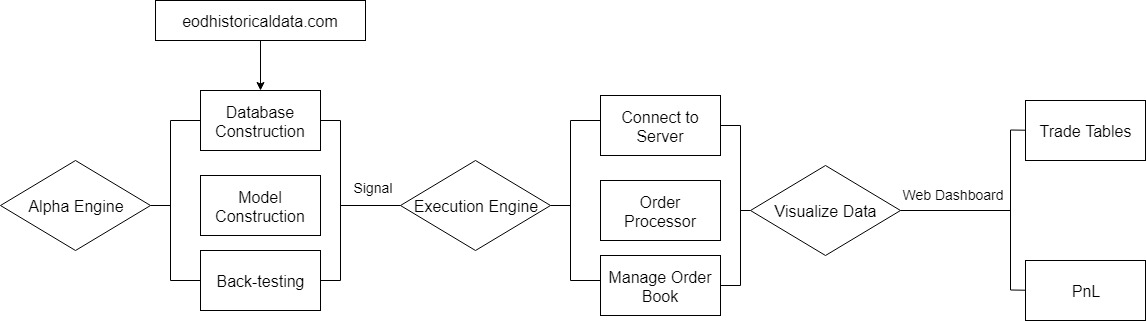
\includegraphics[scale=0.35]{introduction/images/flowchart.jpg}
\caption{Program Design}
\label{fig:flow}
\end{figure}

%
The server is a multi-thread application which coordinates among all the client applications. Its main purposes are 1) messaging among all the participants, 2) maintain a market participant list, and the list of stocks traded by participants, and 3) generate a consolidated order book for all the participants. The client application, also a multi-threading application in network-oriented environment, will communicate with the server. Each application will implement required messages in json format. 

%
Moreover, 1) The sender and receiver threads will support TCP/IP protocol and through Internet sockets;
2) The sender and receiver threads must achieve data synchronization using event and queue;
3) the application will handle direct market data feeds in json format for historical and real-time data from eodhistoricaldata.com;
4) the application will have an integrated database for data persistence. The database we use is sqlite3. We implement tables and SQL statements for our own model buildup, as well as back testing.
5) We will implement a trading model.
6) We manage our own order books and calculate P/L.

%
The trading model is a pairs trading model on stocks in SP500. We use machine learning techniques in selecting pairs. Specifically, we use PCA to reduce dimensions and then DBSCAN clustering to group stocks. We then identify pairs within clusters to implement dollar neutral Bollinger Band pairs trading strategy. Finally, we construct a portfolio with pairs equally weighted. We achieve a 2.5 Sharpe ratio backtested in 2018. However, we can potentially lose money when we trade in simulated market using client/server infrastructure we built.

%
We proceed as follows. In Chapter 2: Background, we provide some backgrounds in pairs trading model and machine learning techniques we used. Chapter 3: Data, we describe how we retrieve, parse and store data into database. In Chapter 4: Trading Model, we describe our trading logic, how we train, build and backtest our model. In Chapter 5: Client/Server, we provide details of client server infrastructure and how they communicate. In Chapter 6: Simulated Trade, we explain how we implement trading strategy to trade in client/server infrastructure. In Chapter 7: Performance Analysis, we show our performance of backtest and simulated trade results and how we move the visualization to web dashboard using flask. At last, we have Chapter 8: Conclusion and appendix where source codes will be provided.

%
%!TEX root = ../thesis.tex
\chapter{Background}
\label{chap:background}
\nocite{*}


\section{Pairs Trading}

Pairs trading is a market-neutral trading strategy that matches a long position with a short position in a pair of highly correlated instruments such as two stocks, exchange-traded funds (ETFs), currencies, commodities or options. Pairs traders wait for weakness in the correlation and then go long the under-performer while simultaneously short selling the over-performer, closing the positions as the relationship returns to statistical norms.\cite{investo:pairs}


\subsection{Cointegration Test}

In order to find pairs to trade in pairs trading, we look for cointegrated relationship in pairs. A pair is cointegrated if individual instruments are of same order and the linear combination of them is stationary. We test stationarity of the linear combination of the pair, say \(y_t\). Stationarity is referred as weak stationarity in this case that a series is stationary if the mean and autocovariance are independent of time and the variance is finite for all times.\cite{wiki:stationarity} We simply regress \(y_t\) on its lagged values \(y_{t-1}\) and find out whether the coefficient \(\phi\) is 1 or not. Consider autoregressive process of order 1, AR(1), as shown:\cite{study:coint}
\begin{equation}
y_t = \phi y_{t-1} + \epsilon_t
\end{equation}
where \(\epsilon_t\) is white noise error term with mean zero and constant variance. Then,
\begin{equation}
\Delta y_t = \delta y_{t-1} + \epsilon_t
\end{equation}
where \(\Delta\) is first difference and \(\delta = \phi - 1\). If \(\delta = 0\), then \(\Delta y_t = \epsilon_t \), it means \(y_t\) is random walk and non-stationary. Otherwise, it is a stationary process. This is called Dickey-Fuller Test.

Moreoever, we have Augmented Dickey-Fuller (ADF) Test, which allows for higher-order autoregressive processes, as shown:\cite{study:coint}
\begin{equation}
\Delta y_t = \alpha + \beta t + \gamma y_{t-1} + \sum_{j=1}^{p} \delta_j \Delta y_{t-j} + \epsilon_t
\end{equation}

For this model, we test for the null hypothesis as \(H_0: \gamma = 0\) against alternative hypothesis as \(H_1: \gamma < 0\). We reject the null if the test statistic is smaller than critical value of a significance level. 

In this project, we use ADF test to check cointegration of two stock price series. We construct linear combination of two stock price series as:
\begin{equation}
y_t = S_t^1 - a S_t^2
\end{equation}
where \(S_t^1\) and \(S_t^2\) are price series of stock 1 and stock 2.


\subsection{Bollinger Band Strategy}

Bollinger band strategy is typically used in pairs trading to capture profit between upper and lower bands. Upper and lower band are constructed 1-2 standard deviations from the moving average of the series \(y_t\).\cite{pairstrading} There are also many ways of entry and exit, long and short. In our trading model, we long when \(y_t\) crosses down the lower band, short when \(y_t\) crosses up the upper band, where the profit is captured between buy and sell points, as shown in Figure 2.1.

\begin{figure}[h!]
\centering
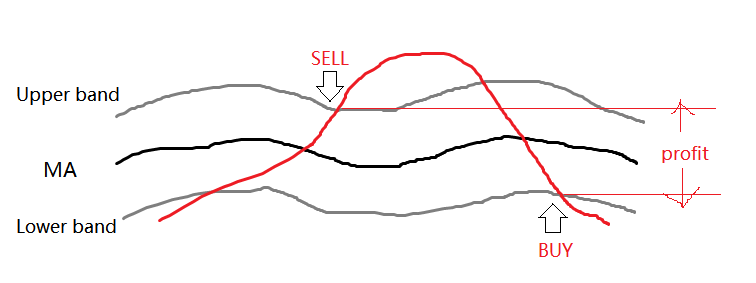
\includegraphics{background/images/bollinger.png}
\caption{Bollinger Band}
\label{fig:bollinger}
\end{figure}



\section{Machine Learning}

\subsection{Principle Component Analysis}

Principle Component Analysis (PCA) is used for reducing the number of variables comprising a dataset while retaining the variability in the data, or identifying hidden patterns in the data, and classifying them according to how much of the information, stored in the data, they account for.\cite{pca} We use PCA for our stock market data for both purposes. 

We take stock price panel data as score matrix \(A\), and coefficient vector \(l\) that generates linear combination on \(A\) which yields principle components \(Y\) of smaller dimension than \(A\). Principle components \(Y\) are independent and each coefficient vector \(l_i\) is required to maximize the variance of its corresponding principle component \(Y_i\), as shown:\cite{pca}
\begin{equation}
\max{Var(Y_i) = l_i^T C l_i}
\end{equation}
\[s.t.\]
\[||l_i^T|| = 1, \forall i\]
\[l_i^T l_j = 0, \forall j\neq i\]
which has Lagrangian form:
\begin{equation}
L(l_i, \lambda_i, \delta) = l_i^T C l_i - \lambda_i(l_i^T l_i - 1) - \delta(l_i^T l_i)
\end{equation}
Maximizing L by taking partial derivatives to 0, we obtain \(C l_i = \lambda_i l_i\), where \(C\) is covariance matrix of \(A\) and \(\lambda_i, l_i\) are corresponding eigenvalues and eigenvectors. 

Therefore, principle components are constructed from eigenvectors of score matrix with score matrix itself: \(Y_i = l_i^T A\).


\subsection{DBSCAN Clustering}

\begin{figure}[h!]
\centering
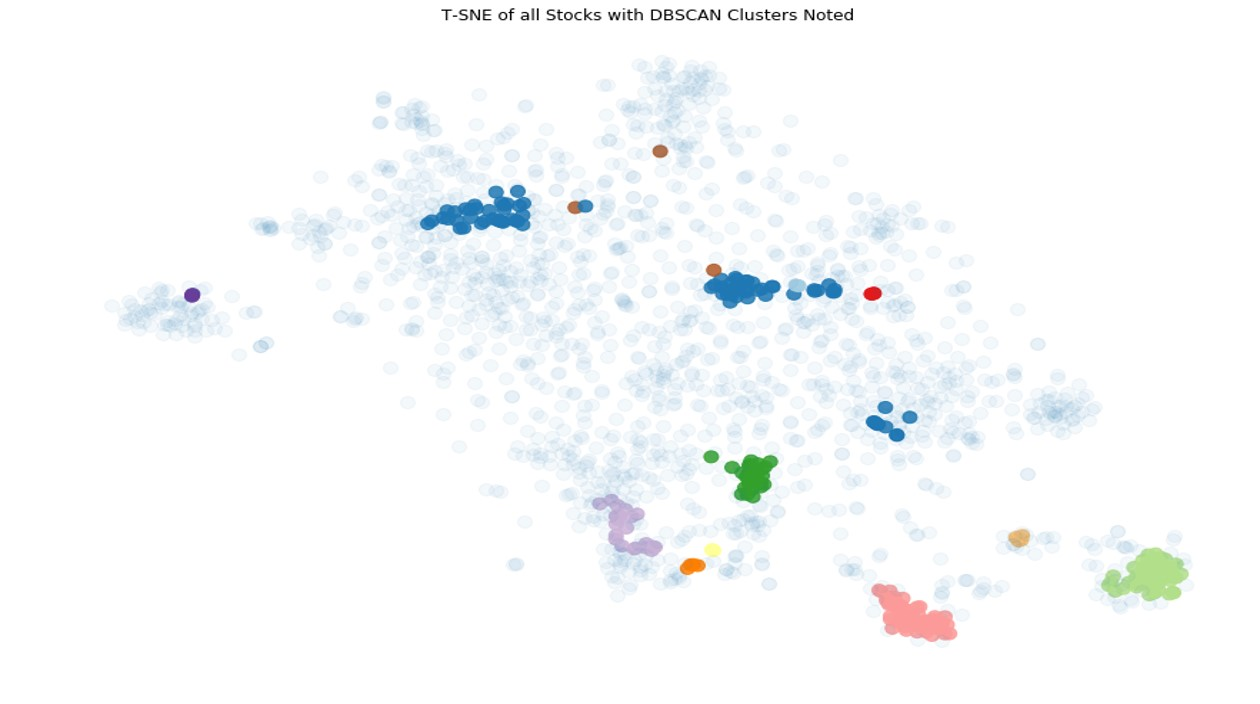
\includegraphics[scale=0.4]{background/images/Clustering.jpg}
\caption{DBSCAN Clustering}
\label{fig:cluster}
\end{figure}

Density-based spatial clustering of applications with noise (DBSCAN) is a density-based clustering non-parametric algorithm: given a set of points in some space, it groups together points that are closely packed together (points with many nearby neighbors).\cite{wiki:dbscan} Unlike normal clustering method that group all points, DBSCAN does not group outliers that lie alone in low-density regions. Another characteristic of DBSCAN is that it is likely to produce different clusters at each run. An example is shown in Figure 2.1.

DBSCAN has two important hyperparameters. Minimum sample size is minimum number of points in a group. Distance parameter is largest distance between points in a group. We pick \( \epsilon = 1.8, min samples = 3\) to get a reasonable number of resulting clusters, which is about 8 clusters.


%
%!TEX root = ../thesis.tex
\chapter{Data}
\label{chap:data}


\section{Data Information}

\subsection{Data Tables}
\begin{enumerate}
    \item "TickerName": stock market data from eodhistoricaldata and are in json format, shown in figure 3.2 includes symbol, date, open, high, low, close, adjusted close, volume from 2014-01-01 to recent, where only adjusted close price is used in our trading model.
    \item "sp500": SP500 constituent data from pkgstore.datahub.io in json format, shown in figure 3.1, which includes name, sector and symbol.
    \item "stockpairs": stock pairs constituent data from training model, which includes ticker1 and ticker2 in pairs, score that represent the strength of cointegration, profit and loss for the pair in backtesting.
    \item "pairprices": stock pairs price data with adjusted close price of each pair from stock market data, residuals from pair prices regression, and bollinger band constructed from residuals.
    \item "trades": trades data that record pair, date, price, quantity and PnL of trade status everyday.
\end{enumerate}

\subsection{Data Retrieval}
We first put SP500 constituent data into database, then retrieve data from each ticker from SP500 and also SP500 index price.

\begin{figure}
\centering
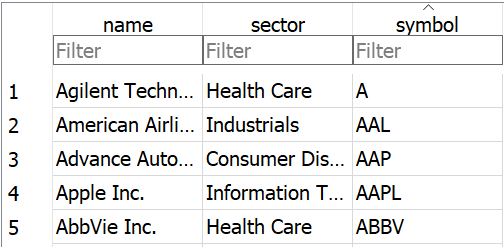
\includegraphics[scale=0.6]{data/images/sp500table.png}
\caption{Table: SP500 Constituents}
\label{fig:sp500}
\end{figure}

\begin{figure}
\centering
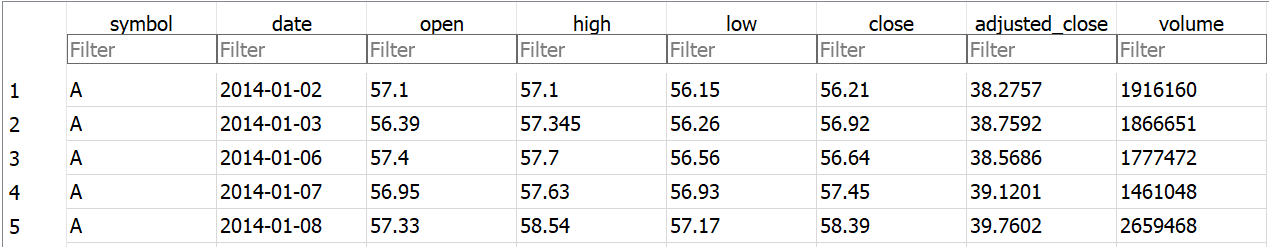
\includegraphics[scale=0.6]{data/images/A.png}
\caption{Table: Stock A}
\label{fig:stockA}
\end{figure}

Function get\_daily\_data() takes in ticker name, start date, end date, data url, api key to get market data for one stock starting from start date to end date. Python packpage urlopen is used to open url and data is parsed from json format to dictionary then to pandas dataframe in Function download\_stock\_data(). Then, the dataframe is stored in SQLite in this function. These functions are shown in Figure 3.3 and 3.4.

\begin{figure}
\centering
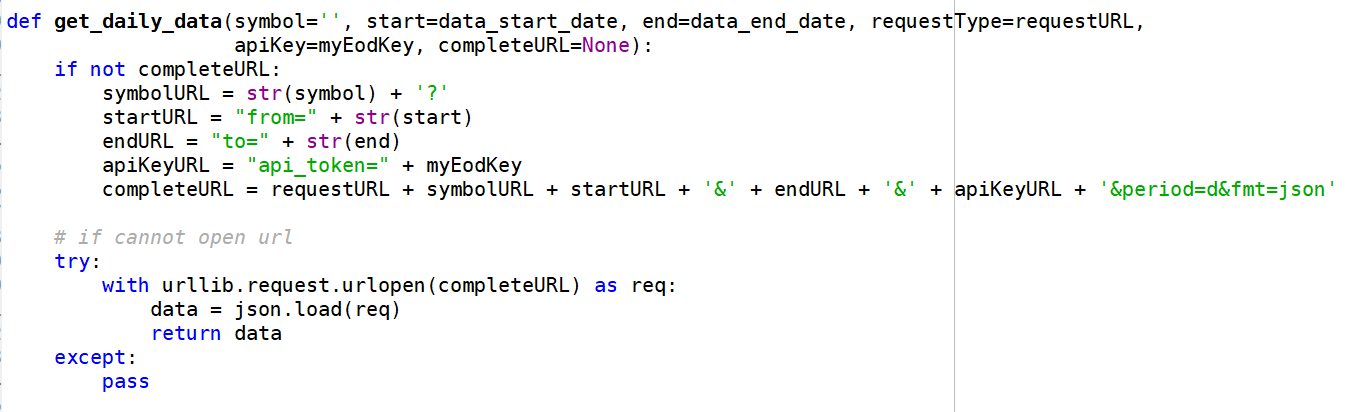
\includegraphics[scale=0.6]{data/images/getdailydata.png}
\caption{Function: get\_daily\_data()}
\label{fig:getdailydata}
\end{figure}

\begin{figure}
\centering
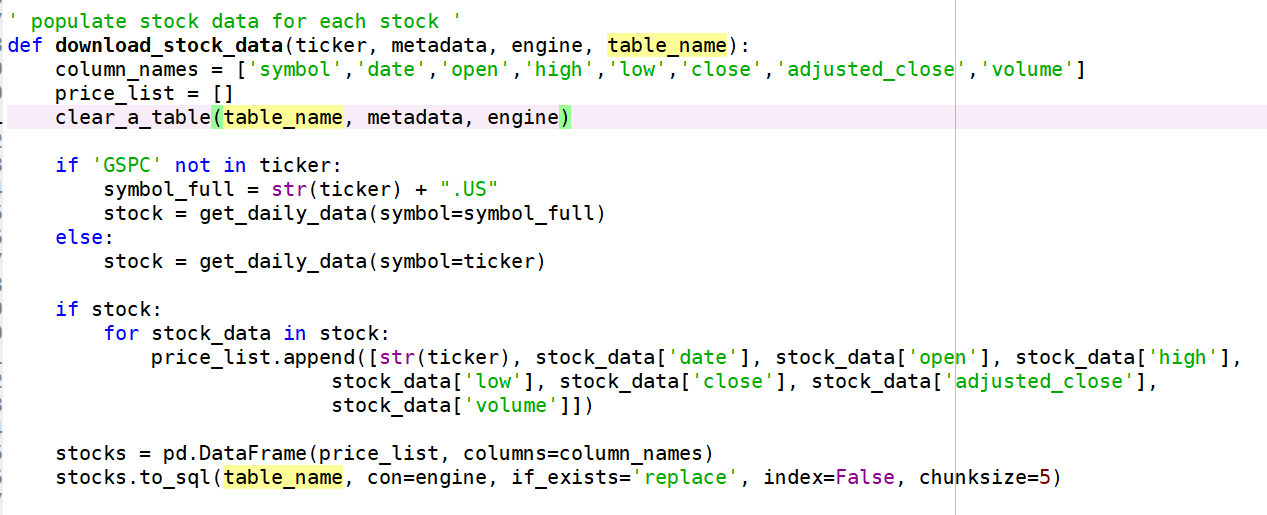
\includegraphics[scale=0.6]{data/images/downloaddata.png}
\caption{Function: download\_stock\_data()}
\label{fig:downloaddata}
\end{figure}


\section{Database Design}

Our database design comprises of 504 tables with two entity relationship, as shown in Figure 3.1. First, each of 500 ticker database with "symbol" and "date" as primary key and "symbol" as foreign key maps to "name" as primary key from sp500 constituents database. Second, table "pairprices" and table "trades" both have "symbol1", "symbol2" that reference to "ticker1", "ticker2" in table stockpairs.

\begin{figure}[h!]
\centering
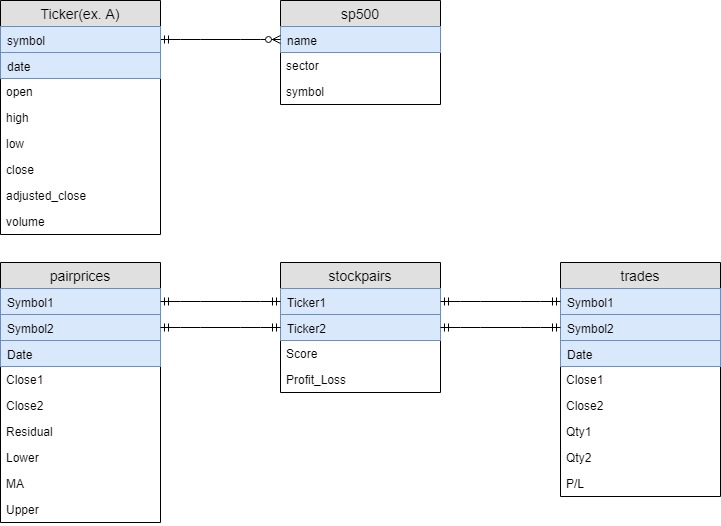
\includegraphics[scale=0.45]{data/images/database.jpg}
\caption{Database Design}
\label{fig:database}
\end{figure}

%
%!TEX root = ../thesis.tex
\chapter{Trading Model}
\label{chap:trading model}

Our trading model is pairs trading model. Pairs are constructed from cointegrated stocks in SP500 stocks in function training\_model(). Then, each pairs is to implement bollinger band strategy in function building\_model(). Later, our trading model will enter function backtesting() with trading signals and corresponding PnL.

\section{Training}

\subsection{Parameters}
\begin{itemize}
    \item training start date: 2014-01-01, training end date: 2018-01-01
    \item capital: 1,000,000 for each pair
    \item cointegration: significance = 0.05
    \item Bollinger Band: standard deviation = 2, moving average period = 10
    \item PCA: principle components = 50, epsilon = 1.8, minimum sample = 3
\end{itemize}

\subsection{Steps}
\begin{enumerate}
    \item 500 stocks price return data of 4 years are reduced to 50 principle components using PCA (background in Section 2.2.1). The resulting dataframe is then in 50 * 500 dimension.
    \item We apply DBSCAN Clustering (background in 2.2.2) to group stocks according to 50 principle components. It will result in 6 to 10 groups with minimum of 3 stocks per group.
    \item Pairs are selected within each group. In each group, every two stocks go through cointegration test (background in 2.1.1). As shown in Figure 4.1, only pairs that pass the test most significantly (smallest p-value, or largest t-statistics) in each group are selected. Information about pairs are stored in table "stockpairs". As shown in Figure 4.2, all pairs have large score (t-statistics).
    \item We then regress one stock price series to another stock price series for each pair using training data. Residual is then constructed in this way as in Equation (2.4). Later, we build bollinger band using residuals (background in Section 2.1.2). Pairs prices, residuals and bollinger bands data are stored in table "pairprices". 
\end{enumerate}

\begin{figure}
\centering
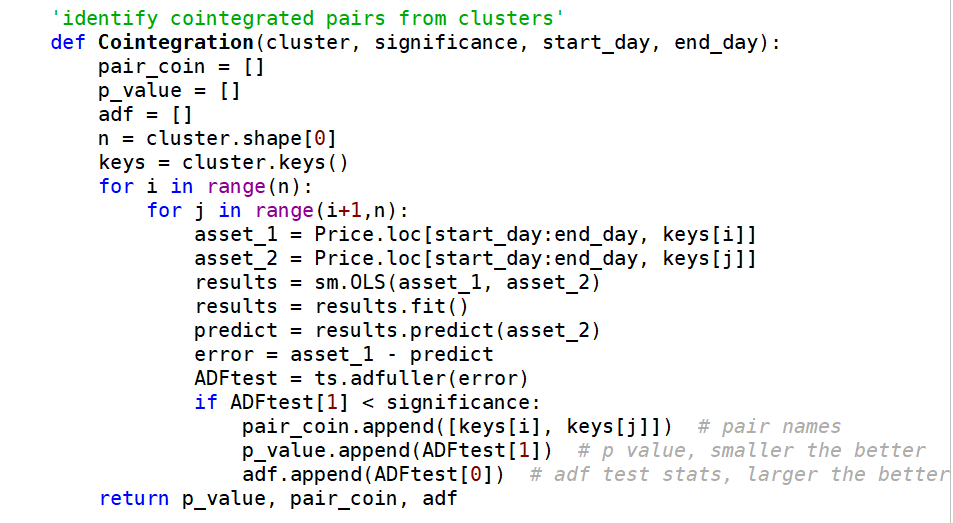
\includegraphics[scale=0.6]{model/images/cointegration.png}
\caption{Function: Cointegration()}
\label{fig:cointegration}
\end{figure}

\begin{figure}[h!]
\centering
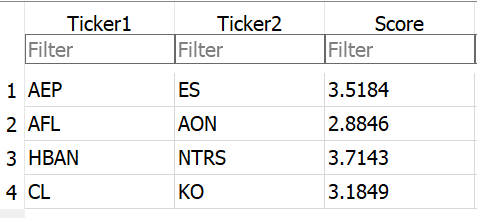
\includegraphics[scale=0.8]{model/images/stockpairs.png}
\caption{Table: Stockpairs}
\label{fig:stockpairs}
\end{figure}




\section{Backtesting}

We backtest from 2018-01-01 to 2019-01-01 for one year. A class is constructed for each stock pair shown in Figure 4.3, where trade is created with stock pair data of each day and is updated if there is a trading signal. Each pair is assigned with equal capital and is market neutral. Profit and loss is also calculated daily according current position and price. Backtesting result is stored in table "trades".


\begin{figure}[h!]
\centering
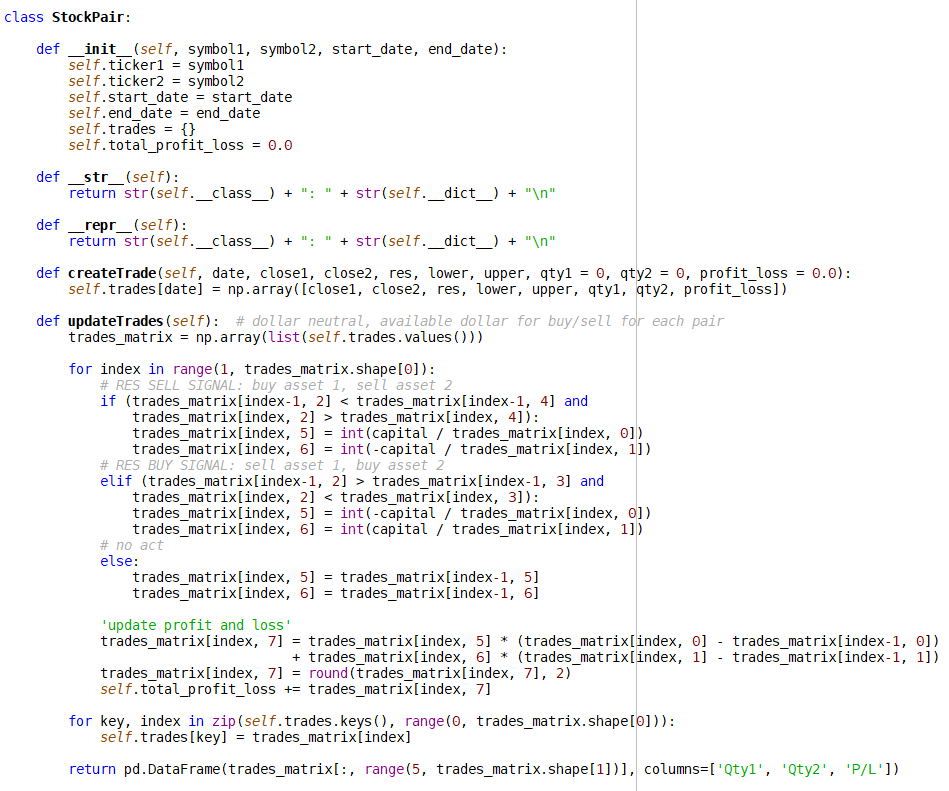
\includegraphics[scale=0.8]{model/images/class.png}
\caption{Class: StockPair}
\label{fig:class}
\end{figure}



%
%!TEX root = ../thesis.tex
\chapter{Client Server}
\label{chap:client server}


The sender and receiver threads will support TCP/IP protocol and through Internet sockets. Server will wait for connection from client, will receive and process messages from client, and will process the request and send back response if client ask for. Socket diagram is shown in Figure 5.1.

\begin{figure}[h!]
\centering
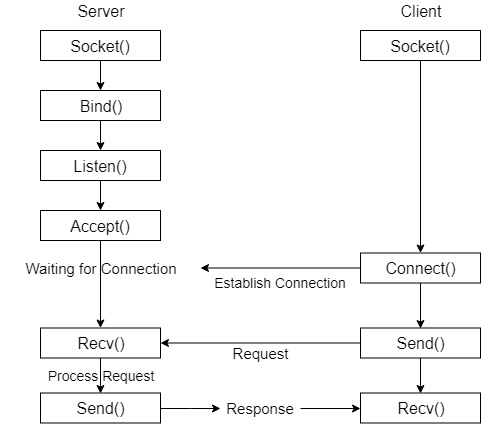
\includegraphics[scale=0.5]{client_server/images/socket.jpg}
\caption{Socket Diagram}
\label{fig:socket}
\end{figure}

The sender and receiver threads achieve data synchronization using event and queue. When the client sends a request message to the server, server returns a message queue while the client is waiting for it. Whenever this event is set, data in queue  will be available to the client. This synchronization process is shown in Figure 5.2.

\begin{figure}[h!]
\centering
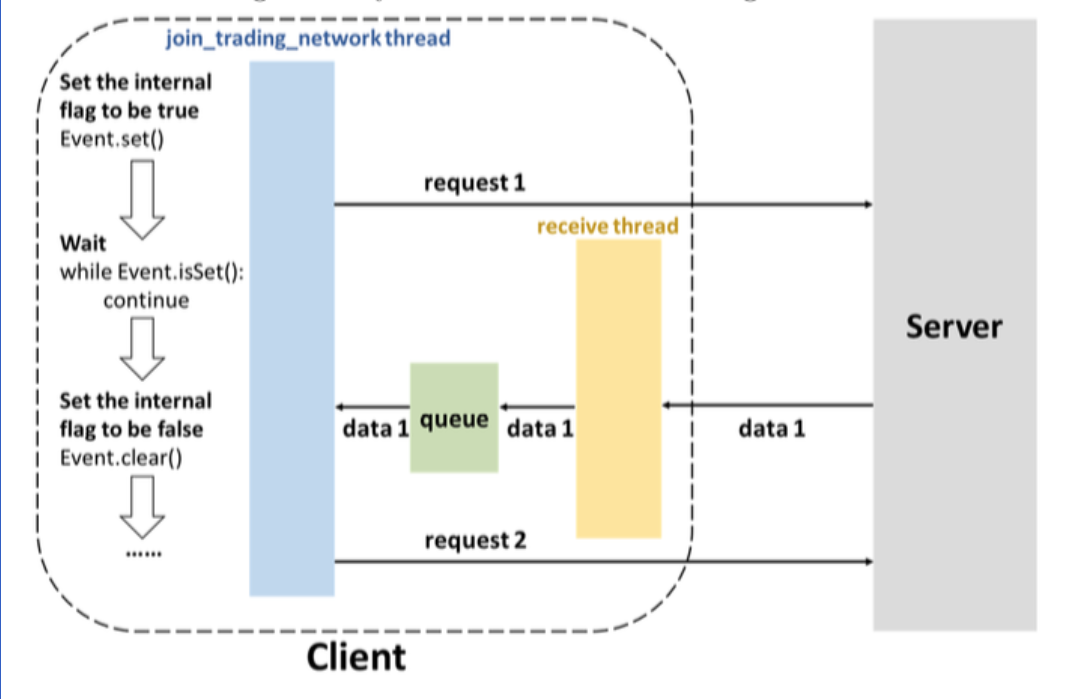
\includegraphics[scale=0.5]{client_server/images/event.png}
\caption{Synchronization Process Diagram}
\label{fig:synch}
\end{figure}


\section{Order Book}
    
Server will provide consolidated books for 30 trading days: 
\begin{enumerate}
    \item Simulated from market data starting from 1/2/2019.
    \item Order book is consist of: order index, symbol, side (buy or sell), price, quantity, and order status, shown in Figure 5.3.
    \item Each simulated trading date has one new book for every 30 seconds from daily historical data, with buy orders and sell orders simulated from the high and low price from the day, with price step of 0.05 and daily volume randomly distributed cross all price points. 
    \item Each simulated trading day lasts 30 seconds, following by 5 seconds of pending closing phase and 5 seconds of market closed phase before market reopen. There are 5 phases of market: 
    \begin{enumerate}
        \item Not Open, start of simulated trading
        \item Pending Open, 
        \item Open, 30s
        \item Pending Close, 5s
        \item Market Close, 5s
    \end{enumerate}
    \item The book supports partial fill, based on comparison of order quantity and available quantity on the book. The order status could be New, Filled or Partial Filled.
    \item If the market status is pending close, trade price will be worse by 0.01.
    \item All orders placed are limit orders.
\end{enumerate}

\begin{figure}[h!]
\centering
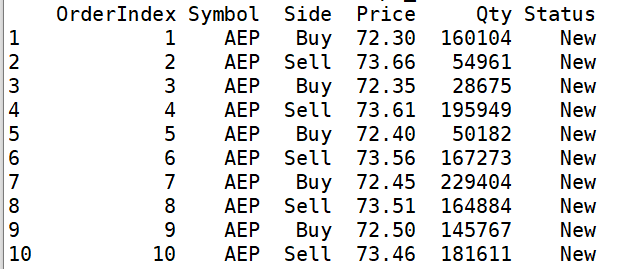
\includegraphics[scale=0.8]{client_server/images/orderbook.png}
\caption{Order Book}
\label{fig:order}
\end{figure}


%
%!TEX root = ../thesis.tex
\chapter{Simulated Trading}
\label{chap:simulated trading}


After training, building, and backtesting the trading model, we will start simulated trading with a "real-time" data feed for 30 days, starting from 01/02/2019. Every 40 seconds, there is a market data feed of another day read from "eodhistoricaldata.com". 

During simulated trading, first, it will logon to that includes a list of stocks from our trading model. Then it will loop to get market status until market open. It will send orders to server only during market open and pending closing. It will get order book information given a list of stocks to access the best available prices. Function get\_orders() tries to get the trading signal using latest data and trained model, then orders are placed and traded if there is any signal on that day. After placing orders, a new day will start every 40 seconds. Then we loop to get market status and repeat this process again.

Finally, when 30 days passed, we quit client and server connection and start to do trading analysis, which will be published to web dashboard. We design an algorithm to detect the ending of 30-day trading period: we will quit the connection whenever the market status remain in "Close" for more than 150 seconds. 

The flowchart of trading under network setting is shown in Figure 6.1.

\begin{figure}[h!]
\centering
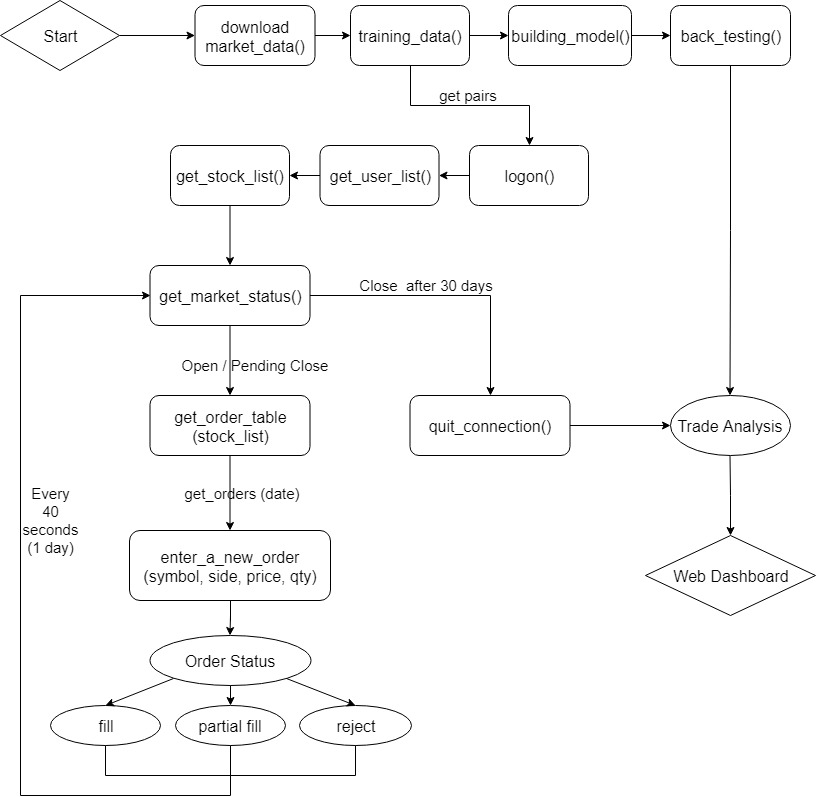
\includegraphics[scale=0.5]{simulated_trading/images/trading.jpg}
\caption{Trading Under Network Setting Flowchart}
\label{fig:trading}
\end{figure}

%
%!TEX root = ../thesis.tex
\chapter{Performance Analysis}
\label{chap:performance analysis}

\section{PnL}
According to Figure 6.1, after both backtesting and simulated trading, we have trading analyses that will be displayed on the web dashboard. Figure 7.2 shows the backtesting result. We can see that backtested from 2018 to 2019, we have a profit of over 1 million, which is about 25\% profit, starting with 1 million capital for each pair and 4 millions in total. All 4 pairs trades are profitable and the hit ratio is 100\%. The maximum drawdown is about only 3\%. The resulting Sharpe ratio is 2.5.

Cummulative PnL plot is also shown in Figure 6.2. Performance of our pairs trading model is much better than SP500 performance. The backtesting result shows that our trading model is very profitable, which is a contrast to our simulated trading result in Figure 6.4. There are several reasons that result in huge losses. First and the most important, our pairs trading model fails since pairs have different relationships during the first month of 2019 than the training data. SP500 index movement in 2018 is quite mean-reverting, where its constituents might also have stable relationships in this year. However, SP500 index at the start of 2019 is more momentum, where its constituents are likely to result in different relationships than in 2018. Second, we have flaws in our design of order book and order matching algorithm. Third, our trading model does not have stop loss. Further discussions of these issues and potential improvements are in conclusion.

\begin{figure}[h!]
\centering
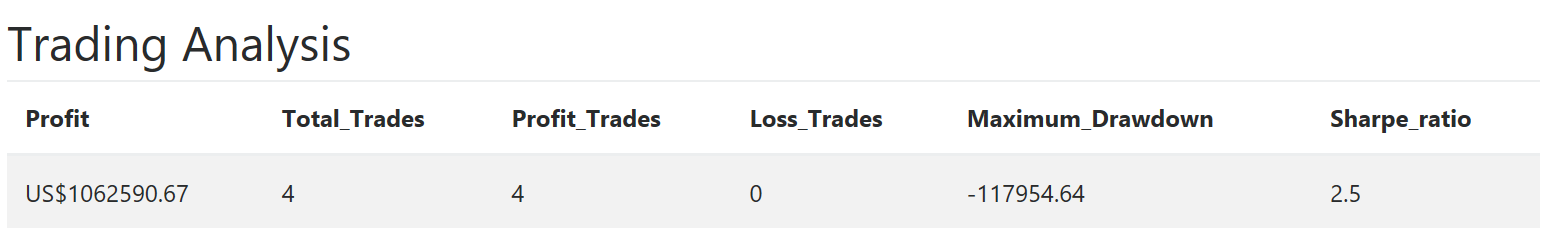
\includegraphics[scale=0.5]{performance_analysis/images/pnl1.png}
\caption{Backtesting Statistics}
\label{fig:backteststats}
\end{figure}

\begin{figure}
\centering
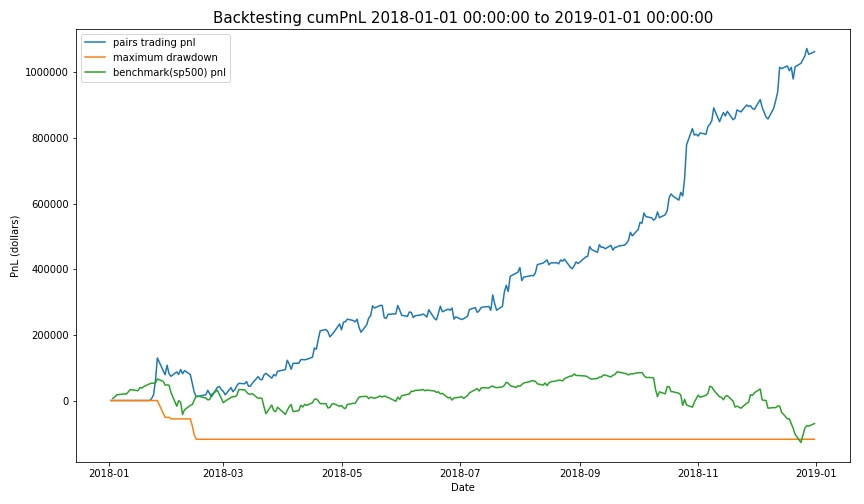
\includegraphics[scale=0.45]{performance_analysis/images/backtest_pnl.jpg}
\caption{Backtesting PnL}
\label{fig:backtest}
\end{figure}

\begin{figure}
\centering
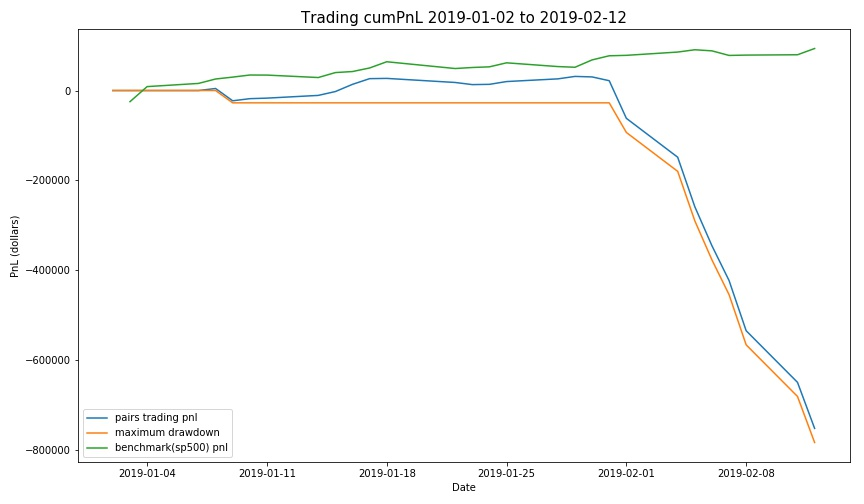
\includegraphics[scale=0.45]{performance_analysis/images/trade_pnl.jpg}
\caption{Simulated Trading PnL}
\label{fig:trading}
\end{figure}



\section{Web Dashboard}

Our web dashboard is built through flask. There are several modules on the web dashboard:
\begin{itemize}
    \item Home Page: displays our pairs trading strategy logic, shown in Figure 7.4;
    \item Stock Pairs: displays Table stockspairs;
    \item Building Model: displays Table pairprices;
    \item Back Testing: displays Table trades;
    \item Trading Analysis: displays performance analysis table and plotted PnL for backtesting result;
    \item Real Trading: displays performance analysis table and plotted PnL for simulated tradingg result;
\end{itemize}

Whenever a module button is clicked on the page, the program will run on the server/client side and the display will show when the process is finished. Each module has to run in order. For "Real Trading" module, it will wait for over 10 minutes until the performance result shows on the page. 

Flask will run on the main thread with the client side. We have another thread called client thread that will do simulated trading part with client/server communication. To do that, we need a global variable "bClientThreadStarted" to keep track if client thread start. It is set to false initially, and to true whenever simulated trading starts. The main thread will wait for client thread finishes to continue.

\begin{figure}
\centering
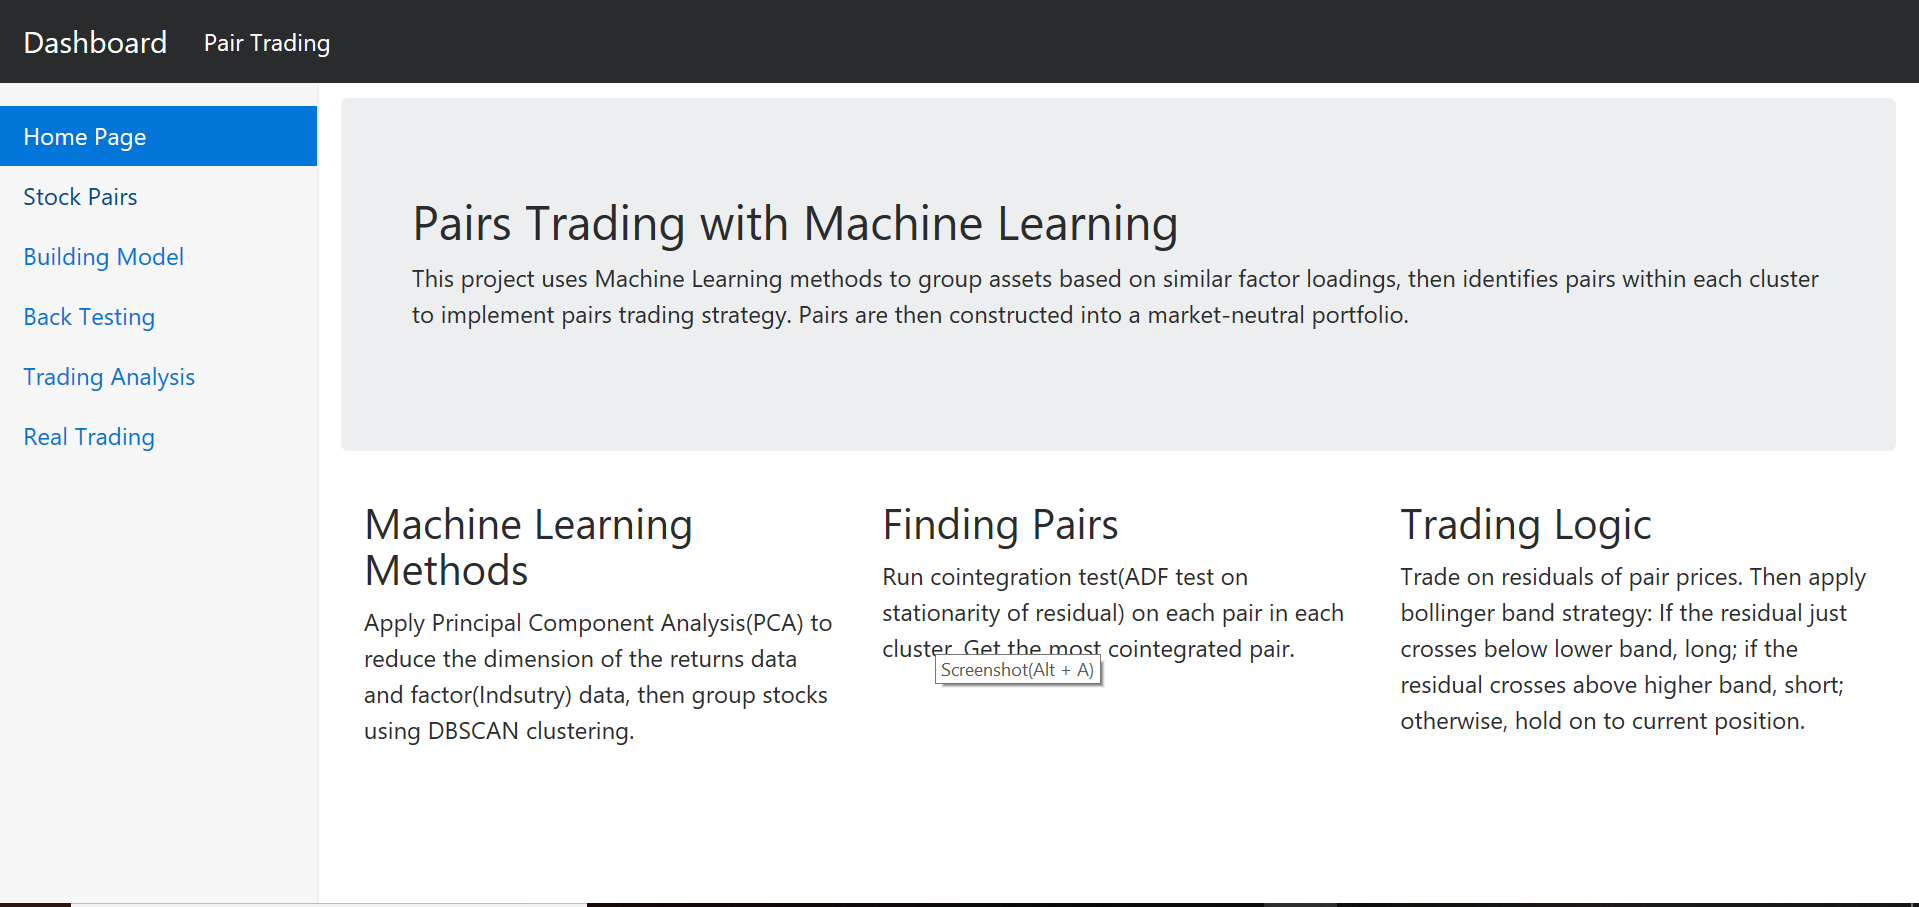
\includegraphics[scale=0.4]{performance_analysis/images/dashboard.png}
\caption{Dashboard Home Page}
\label{fig:dashboard}
\end{figure}



%
%!TEX root = ../thesis.tex
\chapter{Conclusions and Future Work}
\label{chap:conclusions}

This capstone project builds a Python platform that can be used to test quantitative trading models in a network setting under client/server infrastructure with performance analysis displayed on web dashboard. From our backtesting and simulated trading results, we see that the performance of simulated trading is much worse than that of backtesting, although backtesting shows that our trading model has a 2.5 Sharpe ratio and 25\% annual return. It concludes that we should be careful in real-time trading even with a profitable model shown in backtesting and we always want to do paper trading before real trading. 

This python platform is a good tool for testing trading models, alerting for potential losses. However, there are limitations. Our assumptions of order book are simple and our simulated trading is not equivalent to paper trading. Paper trading is to trade based on real-time order books with no real money evolved. Our simulated trading has order book that is simulated from historical data and is fixed for each day. Our order book is too simple as compared to a real order book and is lack of real market dynamics. We would need tick level data to actually simulate a real market, for our first improvement that can be done to this project. Furthermore, we can improve our order matching algorithm and allow for market orders. We always place order at the best bid and offer of one order book of that day and it is always filled at this price. While in the real market, the limit order is fulfilled at our price and better, possibly split into different trades. It also has market order that takes many prices to get as much quantity filled as possible. For our pairs trading model, market orders are more reasonable because we are doing dollar neutral strategy and our purpose is to get all quantity of orders filled.

There are also ways to improve our trading model. First, we have many hyperparameters in our trading model, including training and testing time periods, significance level in adjusted dickey fuller test, number of standard deviations and moving average period in bollinger band construction, number of principle components and epsilon in PCA. These hyperparameters can be optimized through cross validation. Second, we can do kalman filter instead of one simple ordinary least square. Third, we should set up stop loss level to prevent losses as in our simulated trading. Fourth, we should also include transaction costs in our model.

%%%%% Appendices start %%%%%%%%%%%%%%%%
%% Comment out the following line if your thesis has no appendix
\appendix
\chapter{Appendix: Code\label{chap:append}}

%New colors defined below
\definecolor{codegreen}{rgb}{0,0.6,0}
\definecolor{codegray}{rgb}{0.5,0.5,0.5}
\definecolor{codepurple}{rgb}{0.58,0,0.82}
\definecolor{backcolour}{rgb}{0.95,0.95,0.92}

%Code listing style named "mystyle"
\lstdefinestyle{mystyle}{
  backgroundcolor=\color{backcolour},   commentstyle=\color{codegreen},
  keywordstyle=\color{magenta},
  numberstyle=\tiny\color{codegray},
  stringstyle=\color{codepurple},
  basicstyle=\tiny,
  breakatwhitespace=false,         
  breaklines=true,                 
  captionpos=b,                    
  keepspaces=true,                 
  numbers=left,                    
  numbersep=5pt,                  
  showspaces=false,                
  showstringspaces=false,
  showtabs=false,                  
  tabsize=2
}

%"mystyle" code listing set
\lstset{style=mystyle}


\section{Platform Client}
\lstinputlisting[language=Python, caption=Platform Client]{appendix/code/client.py}


\section{Platform Server}
\lstinputlisting[language=Python, caption=Platform Client, basicstyle=\tiny]{appendix/code/server.py}



%% Note: If your thesis has more than one appendix, NYU requires a "list of
%% appendices" page before the body of the thesis. I don't provide the tools
%% to create that here, so you're on your own for that one... Sorry.
%\input{app2}

%%%% Input bibliography file %%%%%%%%%%%%%%%
% %% NYU PhD thesis format. Original template created by José Koiller 2007--2008.
%% Updated by Anshul Vikram Pandey with new design guidelines. 2017-2018

%% Use the first of the following lines during production to
%% easily spot "overfull boxes" in the output. Use the second
%% line for the final version.
\documentclass[12pt,draft,letterpaper]{report}
% \documentclass[12pt,letterpaper]{report}
% \documentclass[12pt]{article}

%% Replace the title, name, advisor name, graduation date and dedication below with
%% your own. Graduation months must be January, May or September.
\newcommand{\thesistitle}{Pairs Trading with Machine Learning on Distributed Python Platform}
\newcommand{\thesisauthor}{Yicheng Wang}
\newcommand{\thesisadvisor}{Song Tang}
\newcommand{\graddate}{May 2019} % like January XX, May 20XX, September 20XX

%% If you do not want a dedication, scroll down and comment out
%% the appropriate lines in this file.
%% \newcommand{\thesisdedication}{To all the Ph.D. pursuing brave souls}

%% The following makes chapters and sections, but not subsections,
%% appear in the TOC (table of contents). Increase to 2 or 3 to
%% make subsections or subsubsections appear, respectively. It seems
%% to be usual to use the "1" setting, however.
\setcounter{tocdepth}{1}

%% Sectional units up to subsubsections are numbered. To number
%% subsections, but not subsubsections, decrease this counter to 2.
\setcounter{secnumdepth}{3}

% Setting a gap between page number and text block


%% Page layout (customized to letter paper and NYU requirements):
\setlength{\oddsidemargin}{.6in}
\setlength{\textwidth}{5.8in}
\setlength{\topmargin}{0.5in}
\setlength{\headheight}{0in}
\setlength{\headsep}{0in}
\setlength{\textheight}{8.3in}
\setlength{\footskip}{.5in}

%% Use the following commands, if desired, during production.
%% Comment them out for final version.
%\usepackage{layout} % defines the \layout command, see below
%\setlength{\hoffset}{-.75in} % creates a large right margin for notes and \showlabels

%% Controls spacing between lines (\doublespacing, \onehalfspacing, etc.):
\usepackage{setspace}

%
%% \usepackage{amsmath}
%% \usepackage{amssymb}
\usepackage{xspace}
\usepackage{algorithmic}
\usepackage{algorithm}
\usepackage{microtype}
\usepackage{subfigure}
\usepackage{color}
\usepackage{url}
\usepackage{fancyhdr}
\usepackage[utf8]{inputenc}
\usepackage[english]{babel}
\usepackage[final]{graphicx}
\usepackage[final]{listings}
\usepackage{color}
% \newfloat{algorithm}{t}{lop}

\pagestyle{fancy}
\fancyhf{}
\renewcommand{\headrulewidth}{0pt}
\fancyhead[LE]{}
\fancyhead[RO]{}
\fancyhead[RE]{}
\fancyhead[LO]{}
\fancyfoot[C]{}
\rhead{\thepage}

\fancypagestyle{plain}{%
\fancyhf{}
\rhead{\thepage}
}

\setlength{\headheight}{20pt} 

%% Use the line below for official NYU version, which requires
%% double line spacing. For all other uses, this is unnecessary,
%% so the line can be commented out.
\onehalfspacing % requires package setspace, invoked above

%% Each of the following lines defines the \com command, which produces
%% a comment (notes for yourself, for instance) in the output file.
%% Example:    \com{this will appear as a comment in the output}
%% Choose (uncomment) only one of the three forms:
%\newcommand{\com}[1]{[/// {#1} ///]}       % between [/// and ///].
\newcommand{\com}[1]{\marginpar{\tiny #1}} % as (tiny) margin notes
%\newcommand{\com}[1]{}                     % suppress all comments.



%% Cross-referencing utilities. Use one or the other--whichever you prefer--
%% but comment out both lines for final version.
%\usepackage{showlabels}
%\usepackage{showkeys}
% \pagestyle{headings}

\begin{document}
%% Produces a test "layout" page, for "debugging" purposes only.
%% Comment out for final version.
%\layout % requires package layout (see above, on this same file)
%% Sets page numbering to "roman style" i, ii, iii, iv, etc:

%%%%%% Cover page %%%%%%%%%%%
%% Sets page numbering to "roman style" i, ii, iii, iv, etc:
\pagenumbering{roman}
\thispagestyle{empty}
\begin{center}
{\bfseries 
  {\large\thesistitle}
  \vspace{1in}
  
 {\large {\bf CAPSTONE}}\\
  \vspace{.5in}
  
  \begin{doublespace}
  {\large  
  Submitted in Partial Fulfillment of\\
  % \vspace{.1in}
  the Requirements for\\
  % \vspace{.1in}
  the Degree of\\}
  \end{doublespace}
  \vspace{.5in}
  
  {\large Master of Science (Finance and Risk Engineering)}\\
  \vspace{.5in}
  
  at the \\
  \vspace{.2in}
  
  {\large
  NEW YORK UNIVERSITY\\
  \vspace{-0.05in}
  TANDON SCHOOL OF ENGINEERING\\
  }
  \vspace{.2in}
  
  by
  \vspace{.5in}

  {\large\thesisauthor}
  \vspace{.5in}
  % \vfill

  {\large\graddate}
}

\end{center}

\newpage

%%%%%%%%%%%%%% Ackknowlegment %%%%%%%%%%%%%%%%%
%% Comment out the following lines if you do not want to acknowledge
%% anyone's help...
\section*{Acknowledgements}
\addcontentsline{toc}{section}{Acknowledgements}
%!TEX root = thesis.tex

I would like to extend my sincere gratitude to Prof. Song Tang for his expert guidance and constructive
feedback throughout the course of this project. I appreciate the patience with which he would tackle my
doubts and the time he would spare from his busy schedule to meet during the course of his work-day
to discuss. His inputs to this project are invaluable. I would also like to thank the Finance and Risk
Engineering department at NYU Tandon School of Engineering to give me the opportunity to work on this advanced topic for my
capstone project, during the course of which I learned a lot.

\noindent
\makebox[\textwidth]{\hfill\makebox[3in]{\hfill Yicheng Wang\hfill}}
\makebox[\textwidth]{\hfill\makebox[3in]{\hfill\graddate\hfill}}


\newpage


%%%%%%%%%%%%%% Abstract %%%%%%%%%%%%%%%%%
\section*{}
\begin{center}
{\bfseries 
  %{\large\thesistitle}
  \vspace{.25in}  
  {\bf ABSTRACT}\\
  \vspace{.25in}
}
\end{center}
\addcontentsline{toc}{section}{Abstract}
%!TEX root = thesis.tex

%
This capstone project implements a distributed Python platform that can be used to test quantitative models for trading financial instruments in a network setting under client/server infrastructure. Normally, we backtest locally using past historical data to check the performance of our trading strategies. The performance result, in this case, is usually an illusion of what the actual performance is in real-time trading. We also show in this paper this conclusion by showing that our quantitative trading model performs much worse in the simulated trading than that in backtesting environment. Therefore, we build this Python platform not only for implementing trading strategies and backtesting them historically but also for simulating trades similar to what is in real market, acting as another control before real-time trading.
\newpage

%%%% Table of Contents %%%%%%%%%%%%
\tableofcontents
% \clearpage
% \pagestyle{headings}


%%%%% Body of thesis starts %%%%%%%%%%%%
\pagenumbering{arabic} % switches page numbering to arabic: 1, 2, 3, etc.

%% Introduction. If your thesis has no introduction, or chapter 1 is
%% meant to be the introduction, then comment out the lines below.
%% \section*{Introduction}\addcontentsline{toc}{section}{Introduction}
%\input{intro}

%%If your thesis has different "Parts", use commands such as the following:
%!TEX root = ../thesis.tex
\chapter{Introduction}
\label{chap:introduction}

%
This capstone project does the following several things coded in Python:
it first sets market data retrieval using Unicorn data feed and parses market data in json format to store market data for backtesting in SQLite database; then implements trading logic; sets up Python Client/Server communication and multi-threading and implements real-time feed to simulate real trade; finally displays trading analysis and PnL on web dashboard. The program has to run in order as described. The program design is also shown in flow chart Figure 1.1.

\begin{figure}
\centering
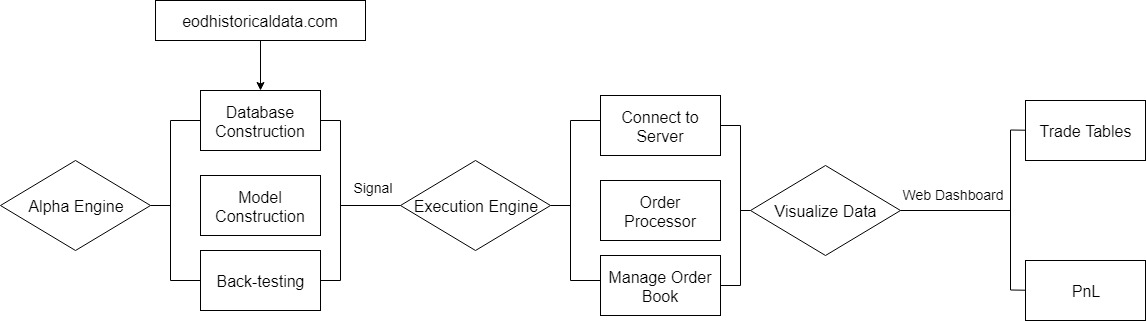
\includegraphics[scale=0.35]{introduction/images/flowchart.jpg}
\caption{Program Design}
\label{fig:flow}
\end{figure}

%
The server is a multi-thread application which coordinates among all the client applications. Its main purposes are 1) messaging among all the participants, 2) maintain a market participant list, and the list of stocks traded by participants, and 3) generate a consolidated order book for all the participants. The client application, also a multi-threading application in network-oriented environment, will communicate with the server. Each application will implement required messages in json format. 

%
Moreover, 1) The sender and receiver threads will support TCP/IP protocol and through Internet sockets;
2) The sender and receiver threads must achieve data synchronization using event and queue;
3) the application will handle direct market data feeds in json format for historical and real-time data from eodhistoricaldata.com;
4) the application will have an integrated database for data persistence. The database we use is sqlite3. We implement tables and SQL statements for our own model buildup, as well as back testing.
5) We will implement a trading model.
6) We manage our own order books and calculate P/L.

%
The trading model is a pairs trading model on stocks in SP500. We use machine learning techniques in selecting pairs. Specifically, we use PCA to reduce dimensions and then DBSCAN clustering to group stocks. We then identify pairs within clusters to implement dollar neutral Bollinger Band pairs trading strategy. Finally, we construct a portfolio with pairs equally weighted. We achieve a 2.5 Sharpe ratio backtested in 2018. However, we can potentially lose money when we trade in simulated market using client/server infrastructure we built.

%
We proceed as follows. In Chapter 2: Background, we provide some backgrounds in pairs trading model and machine learning techniques we used. Chapter 3: Data, we describe how we retrieve, parse and store data into database. In Chapter 4: Trading Model, we describe our trading logic, how we train, build and backtest our model. In Chapter 5: Client/Server, we provide details of client server infrastructure and how they communicate. In Chapter 6: Simulated Trade, we explain how we implement trading strategy to trade in client/server infrastructure. In Chapter 7: Performance Analysis, we show our performance of backtest and simulated trade results and how we move the visualization to web dashboard using flask. At last, we have Chapter 8: Conclusion and appendix where source codes will be provided.

%
%!TEX root = ../thesis.tex
\chapter{Background}
\label{chap:background}
\nocite{*}


\section{Pairs Trading}

Pairs trading is a market-neutral trading strategy that matches a long position with a short position in a pair of highly correlated instruments such as two stocks, exchange-traded funds (ETFs), currencies, commodities or options. Pairs traders wait for weakness in the correlation and then go long the under-performer while simultaneously short selling the over-performer, closing the positions as the relationship returns to statistical norms.\cite{investo:pairs}


\subsection{Cointegration Test}

In order to find pairs to trade in pairs trading, we look for cointegrated relationship in pairs. A pair is cointegrated if individual instruments are of same order and the linear combination of them is stationary. We test stationarity of the linear combination of the pair, say \(y_t\). Stationarity is referred as weak stationarity in this case that a series is stationary if the mean and autocovariance are independent of time and the variance is finite for all times.\cite{wiki:stationarity} We simply regress \(y_t\) on its lagged values \(y_{t-1}\) and find out whether the coefficient \(\phi\) is 1 or not. Consider autoregressive process of order 1, AR(1), as shown:\cite{study:coint}
\begin{equation}
y_t = \phi y_{t-1} + \epsilon_t
\end{equation}
where \(\epsilon_t\) is white noise error term with mean zero and constant variance. Then,
\begin{equation}
\Delta y_t = \delta y_{t-1} + \epsilon_t
\end{equation}
where \(\Delta\) is first difference and \(\delta = \phi - 1\). If \(\delta = 0\), then \(\Delta y_t = \epsilon_t \), it means \(y_t\) is random walk and non-stationary. Otherwise, it is a stationary process. This is called Dickey-Fuller Test.

Moreoever, we have Augmented Dickey-Fuller (ADF) Test, which allows for higher-order autoregressive processes, as shown:\cite{study:coint}
\begin{equation}
\Delta y_t = \alpha + \beta t + \gamma y_{t-1} + \sum_{j=1}^{p} \delta_j \Delta y_{t-j} + \epsilon_t
\end{equation}

For this model, we test for the null hypothesis as \(H_0: \gamma = 0\) against alternative hypothesis as \(H_1: \gamma < 0\). We reject the null if the test statistic is smaller than critical value of a significance level. 

In this project, we use ADF test to check cointegration of two stock price series. We construct linear combination of two stock price series as:
\begin{equation}
y_t = S_t^1 - a S_t^2
\end{equation}
where \(S_t^1\) and \(S_t^2\) are price series of stock 1 and stock 2.


\subsection{Bollinger Band Strategy}

Bollinger band strategy is typically used in pairs trading to capture profit between upper and lower bands. Upper and lower band are constructed 1-2 standard deviations from the moving average of the series \(y_t\).\cite{pairstrading} There are also many ways of entry and exit, long and short. In our trading model, we long when \(y_t\) crosses down the lower band, short when \(y_t\) crosses up the upper band, where the profit is captured between buy and sell points, as shown in Figure 2.1.

\begin{figure}[h!]
\centering
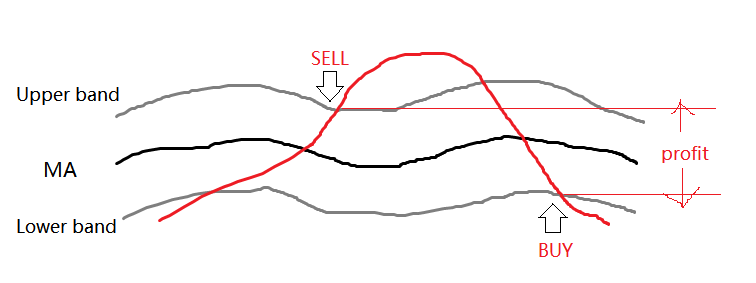
\includegraphics{background/images/bollinger.png}
\caption{Bollinger Band}
\label{fig:bollinger}
\end{figure}



\section{Machine Learning}

\subsection{Principle Component Analysis}

Principle Component Analysis (PCA) is used for reducing the number of variables comprising a dataset while retaining the variability in the data, or identifying hidden patterns in the data, and classifying them according to how much of the information, stored in the data, they account for.\cite{pca} We use PCA for our stock market data for both purposes. 

We take stock price panel data as score matrix \(A\), and coefficient vector \(l\) that generates linear combination on \(A\) which yields principle components \(Y\) of smaller dimension than \(A\). Principle components \(Y\) are independent and each coefficient vector \(l_i\) is required to maximize the variance of its corresponding principle component \(Y_i\), as shown:\cite{pca}
\begin{equation}
\max{Var(Y_i) = l_i^T C l_i}
\end{equation}
\[s.t.\]
\[||l_i^T|| = 1, \forall i\]
\[l_i^T l_j = 0, \forall j\neq i\]
which has Lagrangian form:
\begin{equation}
L(l_i, \lambda_i, \delta) = l_i^T C l_i - \lambda_i(l_i^T l_i - 1) - \delta(l_i^T l_i)
\end{equation}
Maximizing L by taking partial derivatives to 0, we obtain \(C l_i = \lambda_i l_i\), where \(C\) is covariance matrix of \(A\) and \(\lambda_i, l_i\) are corresponding eigenvalues and eigenvectors. 

Therefore, principle components are constructed from eigenvectors of score matrix with score matrix itself: \(Y_i = l_i^T A\).


\subsection{DBSCAN Clustering}

\begin{figure}[h!]
\centering
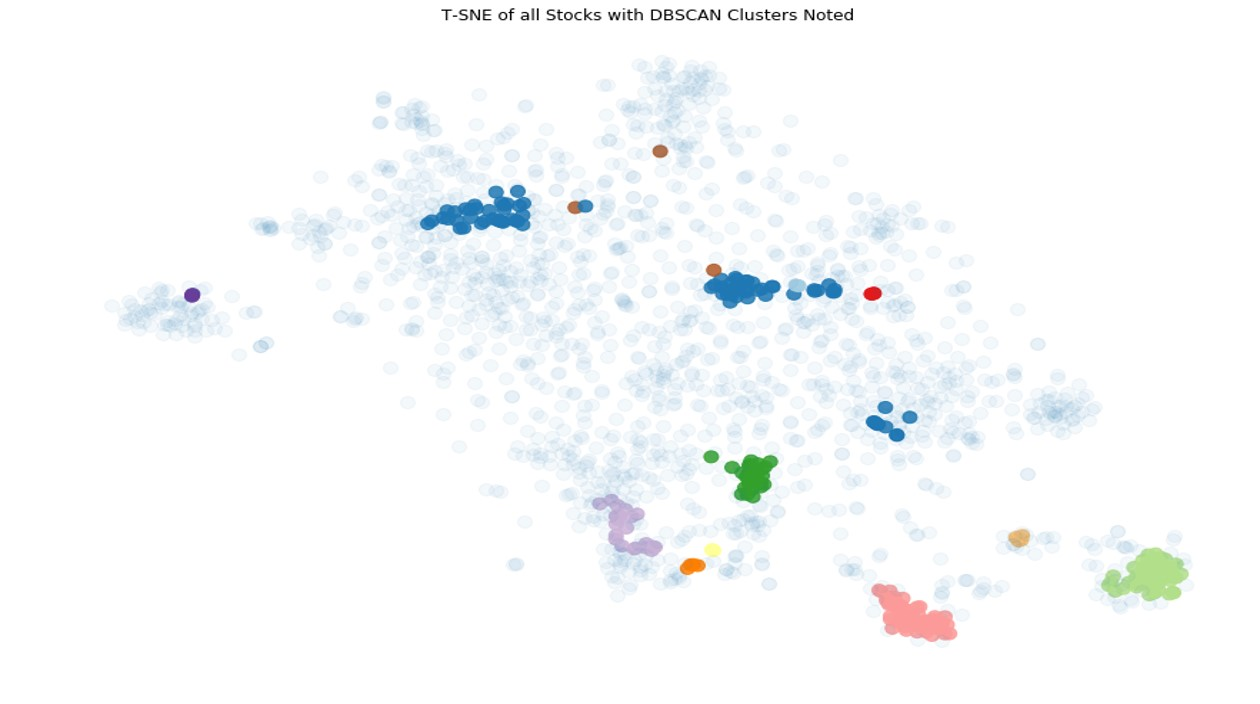
\includegraphics[scale=0.4]{background/images/Clustering.jpg}
\caption{DBSCAN Clustering}
\label{fig:cluster}
\end{figure}

Density-based spatial clustering of applications with noise (DBSCAN) is a density-based clustering non-parametric algorithm: given a set of points in some space, it groups together points that are closely packed together (points with many nearby neighbors).\cite{wiki:dbscan} Unlike normal clustering method that group all points, DBSCAN does not group outliers that lie alone in low-density regions. Another characteristic of DBSCAN is that it is likely to produce different clusters at each run. An example is shown in Figure 2.1.

DBSCAN has two important hyperparameters. Minimum sample size is minimum number of points in a group. Distance parameter is largest distance between points in a group. We pick \( \epsilon = 1.8, min samples = 3\) to get a reasonable number of resulting clusters, which is about 8 clusters.


%
%!TEX root = ../thesis.tex
\chapter{Data}
\label{chap:data}


\section{Data Information}

\subsection{Data Tables}
\begin{enumerate}
    \item "TickerName": stock market data from eodhistoricaldata and are in json format, shown in figure 3.2 includes symbol, date, open, high, low, close, adjusted close, volume from 2014-01-01 to recent, where only adjusted close price is used in our trading model.
    \item "sp500": SP500 constituent data from pkgstore.datahub.io in json format, shown in figure 3.1, which includes name, sector and symbol.
    \item "stockpairs": stock pairs constituent data from training model, which includes ticker1 and ticker2 in pairs, score that represent the strength of cointegration, profit and loss for the pair in backtesting.
    \item "pairprices": stock pairs price data with adjusted close price of each pair from stock market data, residuals from pair prices regression, and bollinger band constructed from residuals.
    \item "trades": trades data that record pair, date, price, quantity and PnL of trade status everyday.
\end{enumerate}

\subsection{Data Retrieval}
We first put SP500 constituent data into database, then retrieve data from each ticker from SP500 and also SP500 index price.

\begin{figure}
\centering
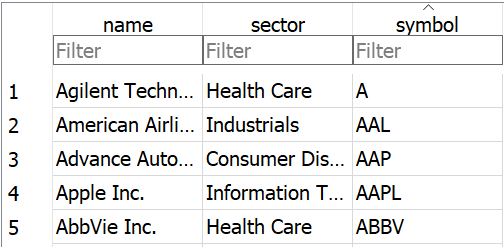
\includegraphics[scale=0.6]{data/images/sp500table.png}
\caption{Table: SP500 Constituents}
\label{fig:sp500}
\end{figure}

\begin{figure}
\centering
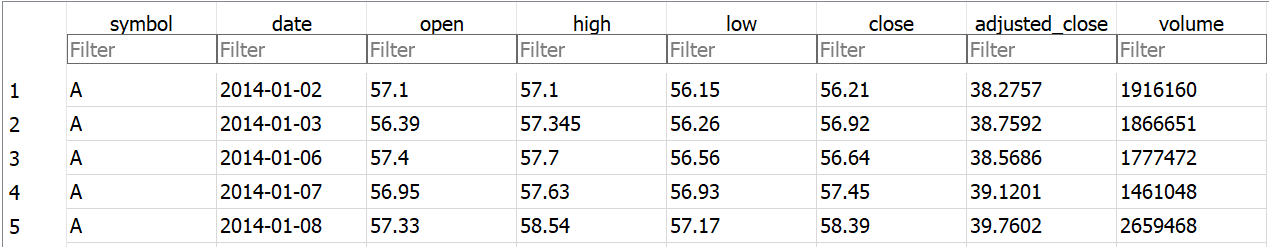
\includegraphics[scale=0.6]{data/images/A.png}
\caption{Table: Stock A}
\label{fig:stockA}
\end{figure}

Function get\_daily\_data() takes in ticker name, start date, end date, data url, api key to get market data for one stock starting from start date to end date. Python packpage urlopen is used to open url and data is parsed from json format to dictionary then to pandas dataframe in Function download\_stock\_data(). Then, the dataframe is stored in SQLite in this function. These functions are shown in Figure 3.3 and 3.4.

\begin{figure}
\centering
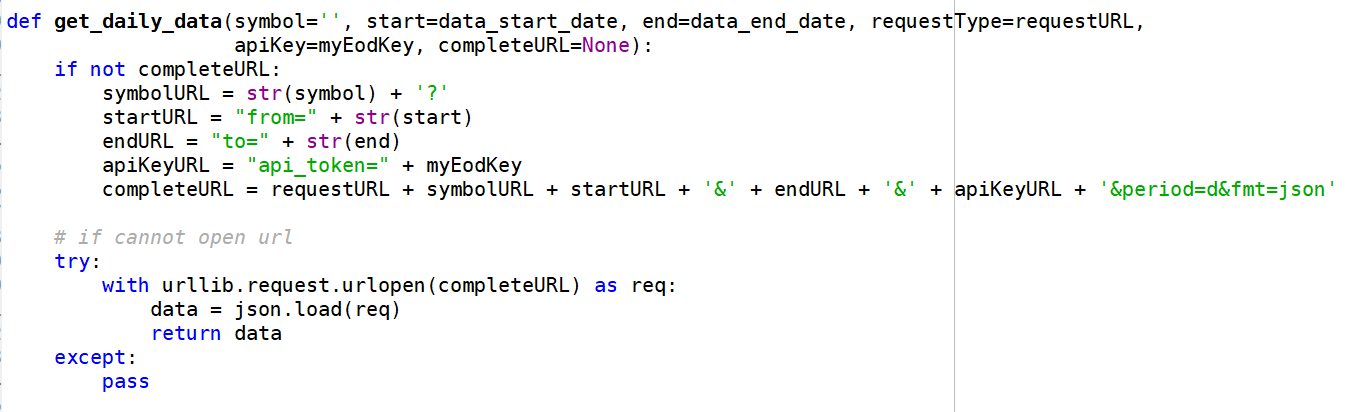
\includegraphics[scale=0.6]{data/images/getdailydata.png}
\caption{Function: get\_daily\_data()}
\label{fig:getdailydata}
\end{figure}

\begin{figure}
\centering
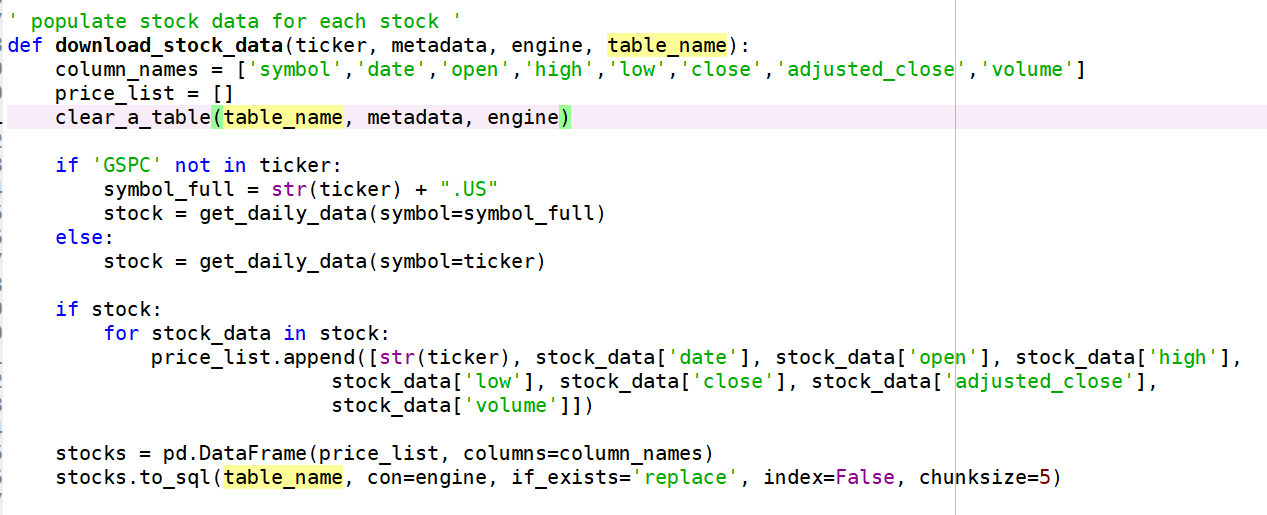
\includegraphics[scale=0.6]{data/images/downloaddata.png}
\caption{Function: download\_stock\_data()}
\label{fig:downloaddata}
\end{figure}


\section{Database Design}

Our database design comprises of 504 tables with two entity relationship, as shown in Figure 3.1. First, each of 500 ticker database with "symbol" and "date" as primary key and "symbol" as foreign key maps to "name" as primary key from sp500 constituents database. Second, table "pairprices" and table "trades" both have "symbol1", "symbol2" that reference to "ticker1", "ticker2" in table stockpairs.

\begin{figure}[h!]
\centering
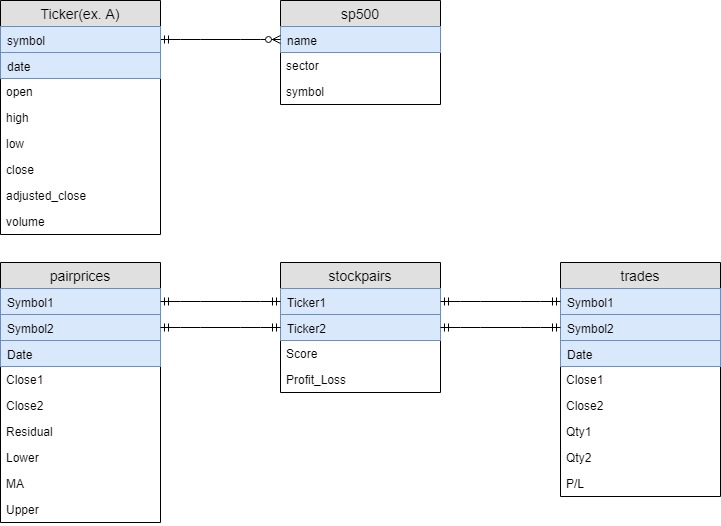
\includegraphics[scale=0.45]{data/images/database.jpg}
\caption{Database Design}
\label{fig:database}
\end{figure}

%
%!TEX root = ../thesis.tex
\chapter{Trading Model}
\label{chap:trading model}

Our trading model is pairs trading model. Pairs are constructed from cointegrated stocks in SP500 stocks in function training\_model(). Then, each pairs is to implement bollinger band strategy in function building\_model(). Later, our trading model will enter function backtesting() with trading signals and corresponding PnL.

\section{Training}

\subsection{Parameters}
\begin{itemize}
    \item training start date: 2014-01-01, training end date: 2018-01-01
    \item capital: 1,000,000 for each pair
    \item cointegration: significance = 0.05
    \item Bollinger Band: standard deviation = 2, moving average period = 10
    \item PCA: principle components = 50, epsilon = 1.8, minimum sample = 3
\end{itemize}

\subsection{Steps}
\begin{enumerate}
    \item 500 stocks price return data of 4 years are reduced to 50 principle components using PCA (background in Section 2.2.1). The resulting dataframe is then in 50 * 500 dimension.
    \item We apply DBSCAN Clustering (background in 2.2.2) to group stocks according to 50 principle components. It will result in 6 to 10 groups with minimum of 3 stocks per group.
    \item Pairs are selected within each group. In each group, every two stocks go through cointegration test (background in 2.1.1). As shown in Figure 4.1, only pairs that pass the test most significantly (smallest p-value, or largest t-statistics) in each group are selected. Information about pairs are stored in table "stockpairs". As shown in Figure 4.2, all pairs have large score (t-statistics).
    \item We then regress one stock price series to another stock price series for each pair using training data. Residual is then constructed in this way as in Equation (2.4). Later, we build bollinger band using residuals (background in Section 2.1.2). Pairs prices, residuals and bollinger bands data are stored in table "pairprices". 
\end{enumerate}

\begin{figure}
\centering
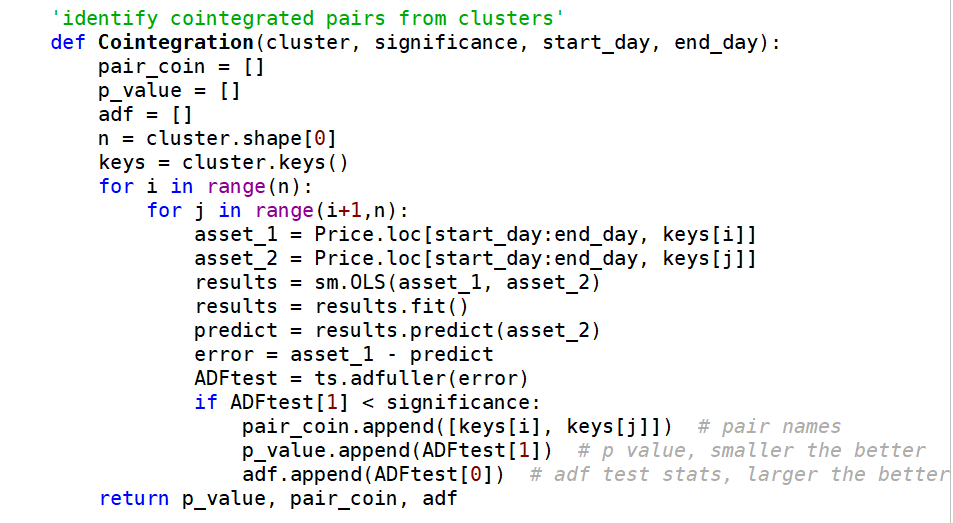
\includegraphics[scale=0.6]{model/images/cointegration.png}
\caption{Function: Cointegration()}
\label{fig:cointegration}
\end{figure}

\begin{figure}[h!]
\centering
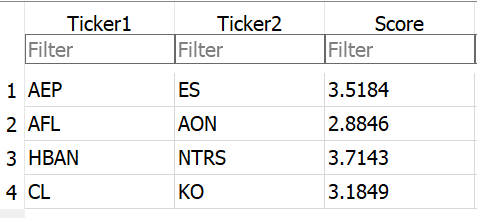
\includegraphics[scale=0.8]{model/images/stockpairs.png}
\caption{Table: Stockpairs}
\label{fig:stockpairs}
\end{figure}




\section{Backtesting}

We backtest from 2018-01-01 to 2019-01-01 for one year. A class is constructed for each stock pair shown in Figure 4.3, where trade is created with stock pair data of each day and is updated if there is a trading signal. Each pair is assigned with equal capital and is market neutral. Profit and loss is also calculated daily according current position and price. Backtesting result is stored in table "trades".


\begin{figure}[h!]
\centering
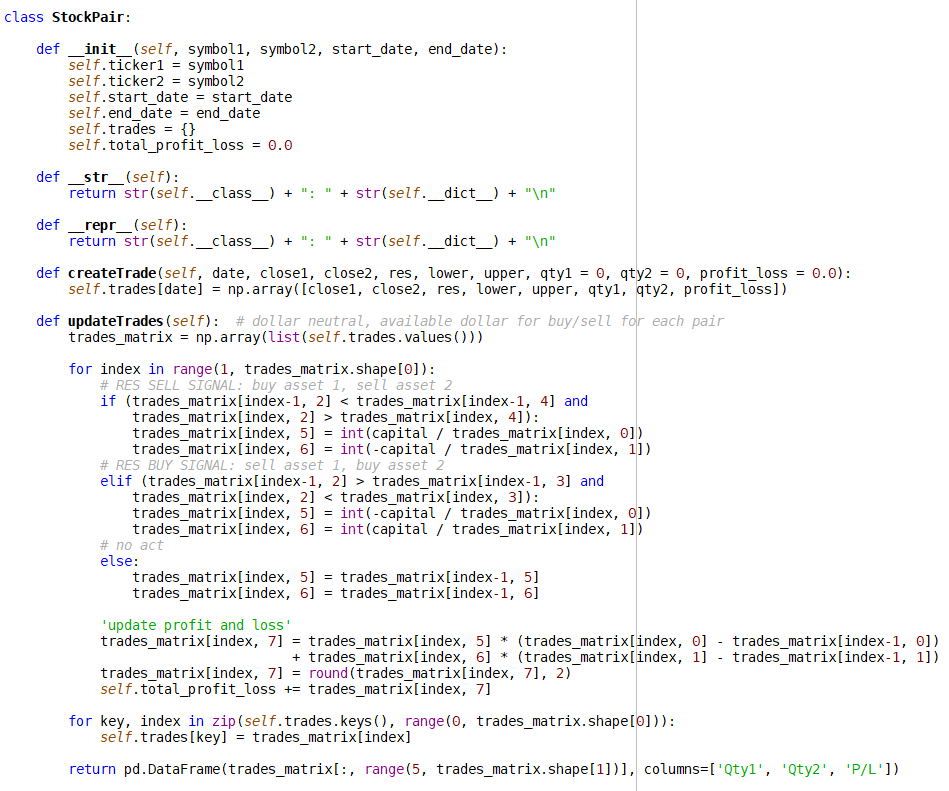
\includegraphics[scale=0.8]{model/images/class.png}
\caption{Class: StockPair}
\label{fig:class}
\end{figure}



%
%!TEX root = ../thesis.tex
\chapter{Client Server}
\label{chap:client server}


The sender and receiver threads will support TCP/IP protocol and through Internet sockets. Server will wait for connection from client, will receive and process messages from client, and will process the request and send back response if client ask for. Socket diagram is shown in Figure 5.1.

\begin{figure}[h!]
\centering
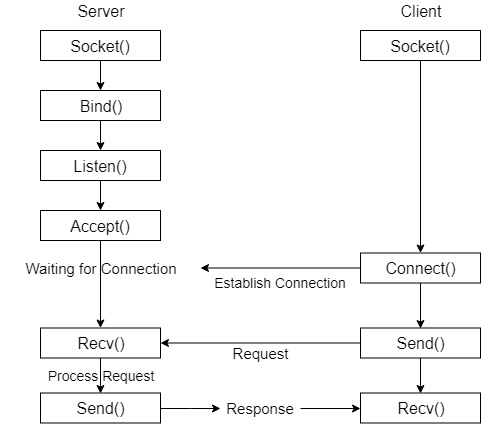
\includegraphics[scale=0.5]{client_server/images/socket.jpg}
\caption{Socket Diagram}
\label{fig:socket}
\end{figure}

The sender and receiver threads achieve data synchronization using event and queue. When the client sends a request message to the server, server returns a message queue while the client is waiting for it. Whenever this event is set, data in queue  will be available to the client. This synchronization process is shown in Figure 5.2.

\begin{figure}[h!]
\centering
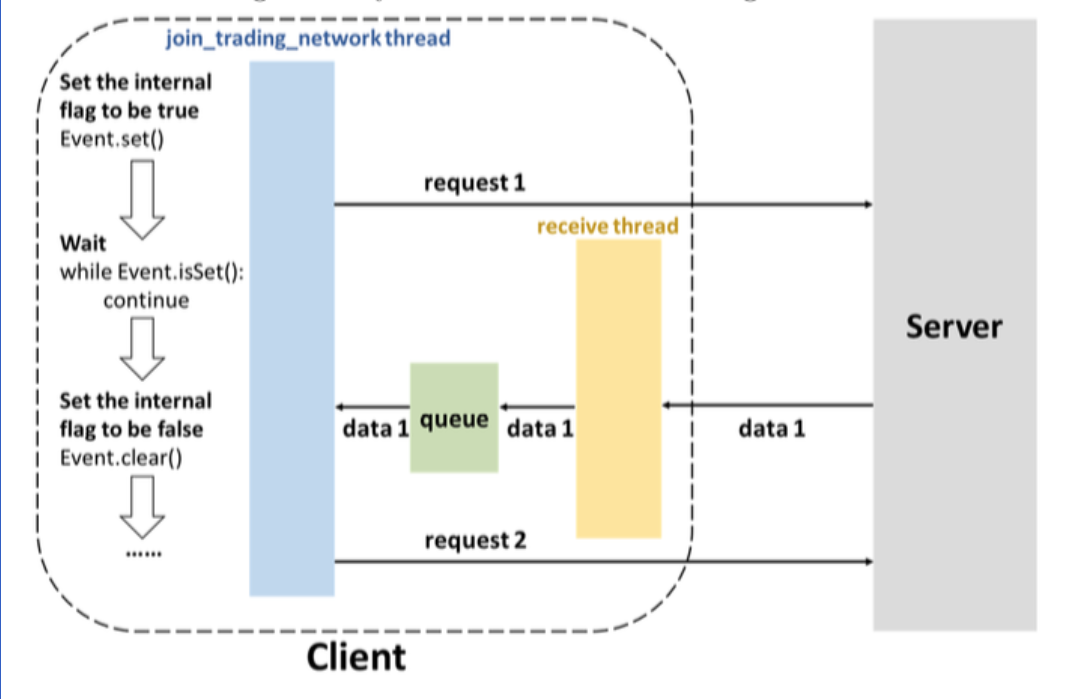
\includegraphics[scale=0.5]{client_server/images/event.png}
\caption{Synchronization Process Diagram}
\label{fig:synch}
\end{figure}


\section{Order Book}
    
Server will provide consolidated books for 30 trading days: 
\begin{enumerate}
    \item Simulated from market data starting from 1/2/2019.
    \item Order book is consist of: order index, symbol, side (buy or sell), price, quantity, and order status, shown in Figure 5.3.
    \item Each simulated trading date has one new book for every 30 seconds from daily historical data, with buy orders and sell orders simulated from the high and low price from the day, with price step of 0.05 and daily volume randomly distributed cross all price points. 
    \item Each simulated trading day lasts 30 seconds, following by 5 seconds of pending closing phase and 5 seconds of market closed phase before market reopen. There are 5 phases of market: 
    \begin{enumerate}
        \item Not Open, start of simulated trading
        \item Pending Open, 
        \item Open, 30s
        \item Pending Close, 5s
        \item Market Close, 5s
    \end{enumerate}
    \item The book supports partial fill, based on comparison of order quantity and available quantity on the book. The order status could be New, Filled or Partial Filled.
    \item If the market status is pending close, trade price will be worse by 0.01.
    \item All orders placed are limit orders.
\end{enumerate}

\begin{figure}[h!]
\centering
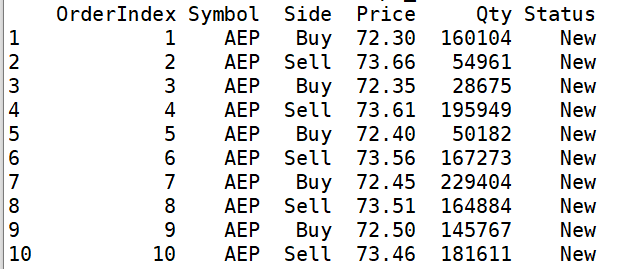
\includegraphics[scale=0.8]{client_server/images/orderbook.png}
\caption{Order Book}
\label{fig:order}
\end{figure}


%
%!TEX root = ../thesis.tex
\chapter{Simulated Trading}
\label{chap:simulated trading}


After training, building, and backtesting the trading model, we will start simulated trading with a "real-time" data feed for 30 days, starting from 01/02/2019. Every 40 seconds, there is a market data feed of another day read from "eodhistoricaldata.com". 

During simulated trading, first, it will logon to that includes a list of stocks from our trading model. Then it will loop to get market status until market open. It will send orders to server only during market open and pending closing. It will get order book information given a list of stocks to access the best available prices. Function get\_orders() tries to get the trading signal using latest data and trained model, then orders are placed and traded if there is any signal on that day. After placing orders, a new day will start every 40 seconds. Then we loop to get market status and repeat this process again.

Finally, when 30 days passed, we quit client and server connection and start to do trading analysis, which will be published to web dashboard. We design an algorithm to detect the ending of 30-day trading period: we will quit the connection whenever the market status remain in "Close" for more than 150 seconds. 

The flowchart of trading under network setting is shown in Figure 6.1.

\begin{figure}[h!]
\centering
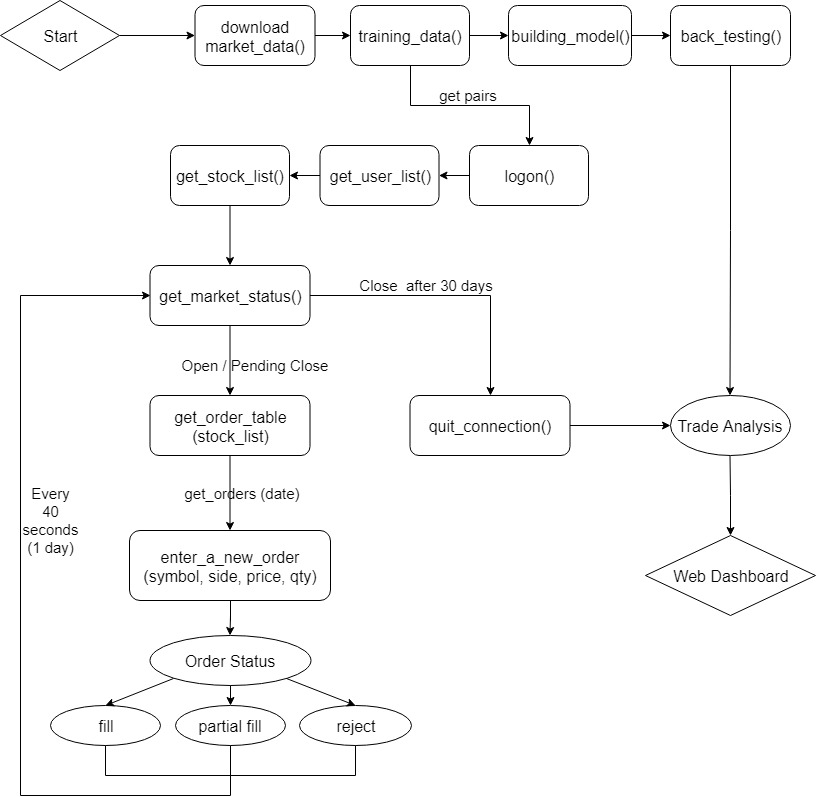
\includegraphics[scale=0.5]{simulated_trading/images/trading.jpg}
\caption{Trading Under Network Setting Flowchart}
\label{fig:trading}
\end{figure}

%
%!TEX root = ../thesis.tex
\chapter{Performance Analysis}
\label{chap:performance analysis}

\section{PnL}
According to Figure 6.1, after both backtesting and simulated trading, we have trading analyses that will be displayed on the web dashboard. Figure 7.2 shows the backtesting result. We can see that backtested from 2018 to 2019, we have a profit of over 1 million, which is about 25\% profit, starting with 1 million capital for each pair and 4 millions in total. All 4 pairs trades are profitable and the hit ratio is 100\%. The maximum drawdown is about only 3\%. The resulting Sharpe ratio is 2.5.

Cummulative PnL plot is also shown in Figure 6.2. Performance of our pairs trading model is much better than SP500 performance. The backtesting result shows that our trading model is very profitable, which is a contrast to our simulated trading result in Figure 6.4. There are several reasons that result in huge losses. First and the most important, our pairs trading model fails since pairs have different relationships during the first month of 2019 than the training data. SP500 index movement in 2018 is quite mean-reverting, where its constituents might also have stable relationships in this year. However, SP500 index at the start of 2019 is more momentum, where its constituents are likely to result in different relationships than in 2018. Second, we have flaws in our design of order book and order matching algorithm. Third, our trading model does not have stop loss. Further discussions of these issues and potential improvements are in conclusion.

\begin{figure}[h!]
\centering
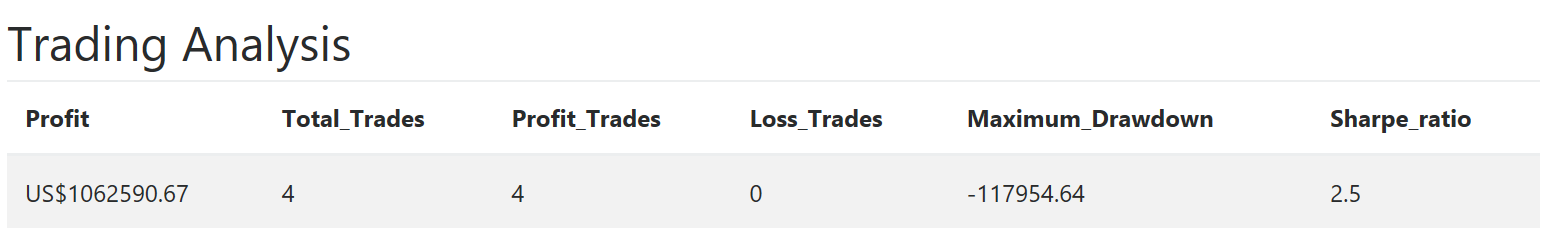
\includegraphics[scale=0.5]{performance_analysis/images/pnl1.png}
\caption{Backtesting Statistics}
\label{fig:backteststats}
\end{figure}

\begin{figure}
\centering
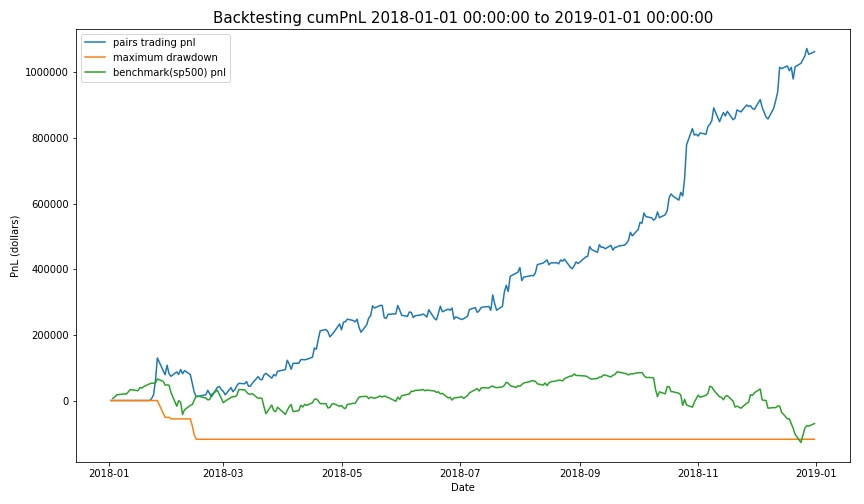
\includegraphics[scale=0.45]{performance_analysis/images/backtest_pnl.jpg}
\caption{Backtesting PnL}
\label{fig:backtest}
\end{figure}

\begin{figure}
\centering
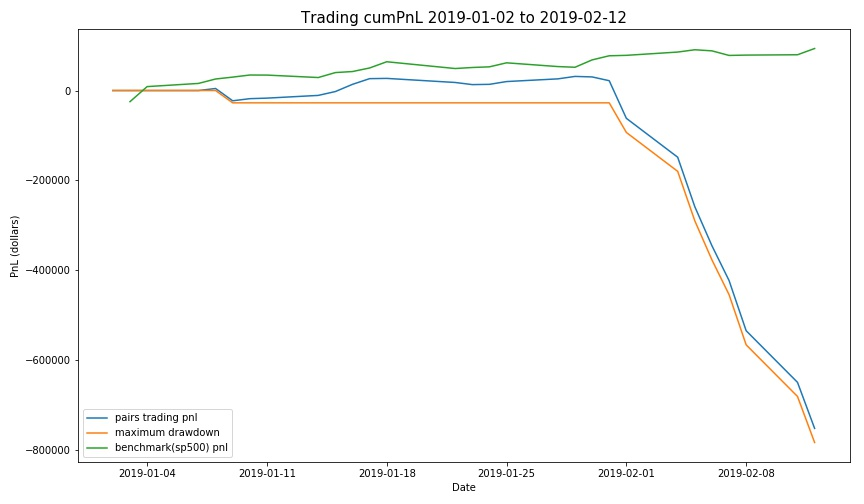
\includegraphics[scale=0.45]{performance_analysis/images/trade_pnl.jpg}
\caption{Simulated Trading PnL}
\label{fig:trading}
\end{figure}



\section{Web Dashboard}

Our web dashboard is built through flask. There are several modules on the web dashboard:
\begin{itemize}
    \item Home Page: displays our pairs trading strategy logic, shown in Figure 7.4;
    \item Stock Pairs: displays Table stockspairs;
    \item Building Model: displays Table pairprices;
    \item Back Testing: displays Table trades;
    \item Trading Analysis: displays performance analysis table and plotted PnL for backtesting result;
    \item Real Trading: displays performance analysis table and plotted PnL for simulated tradingg result;
\end{itemize}

Whenever a module button is clicked on the page, the program will run on the server/client side and the display will show when the process is finished. Each module has to run in order. For "Real Trading" module, it will wait for over 10 minutes until the performance result shows on the page. 

Flask will run on the main thread with the client side. We have another thread called client thread that will do simulated trading part with client/server communication. To do that, we need a global variable "bClientThreadStarted" to keep track if client thread start. It is set to false initially, and to true whenever simulated trading starts. The main thread will wait for client thread finishes to continue.

\begin{figure}
\centering
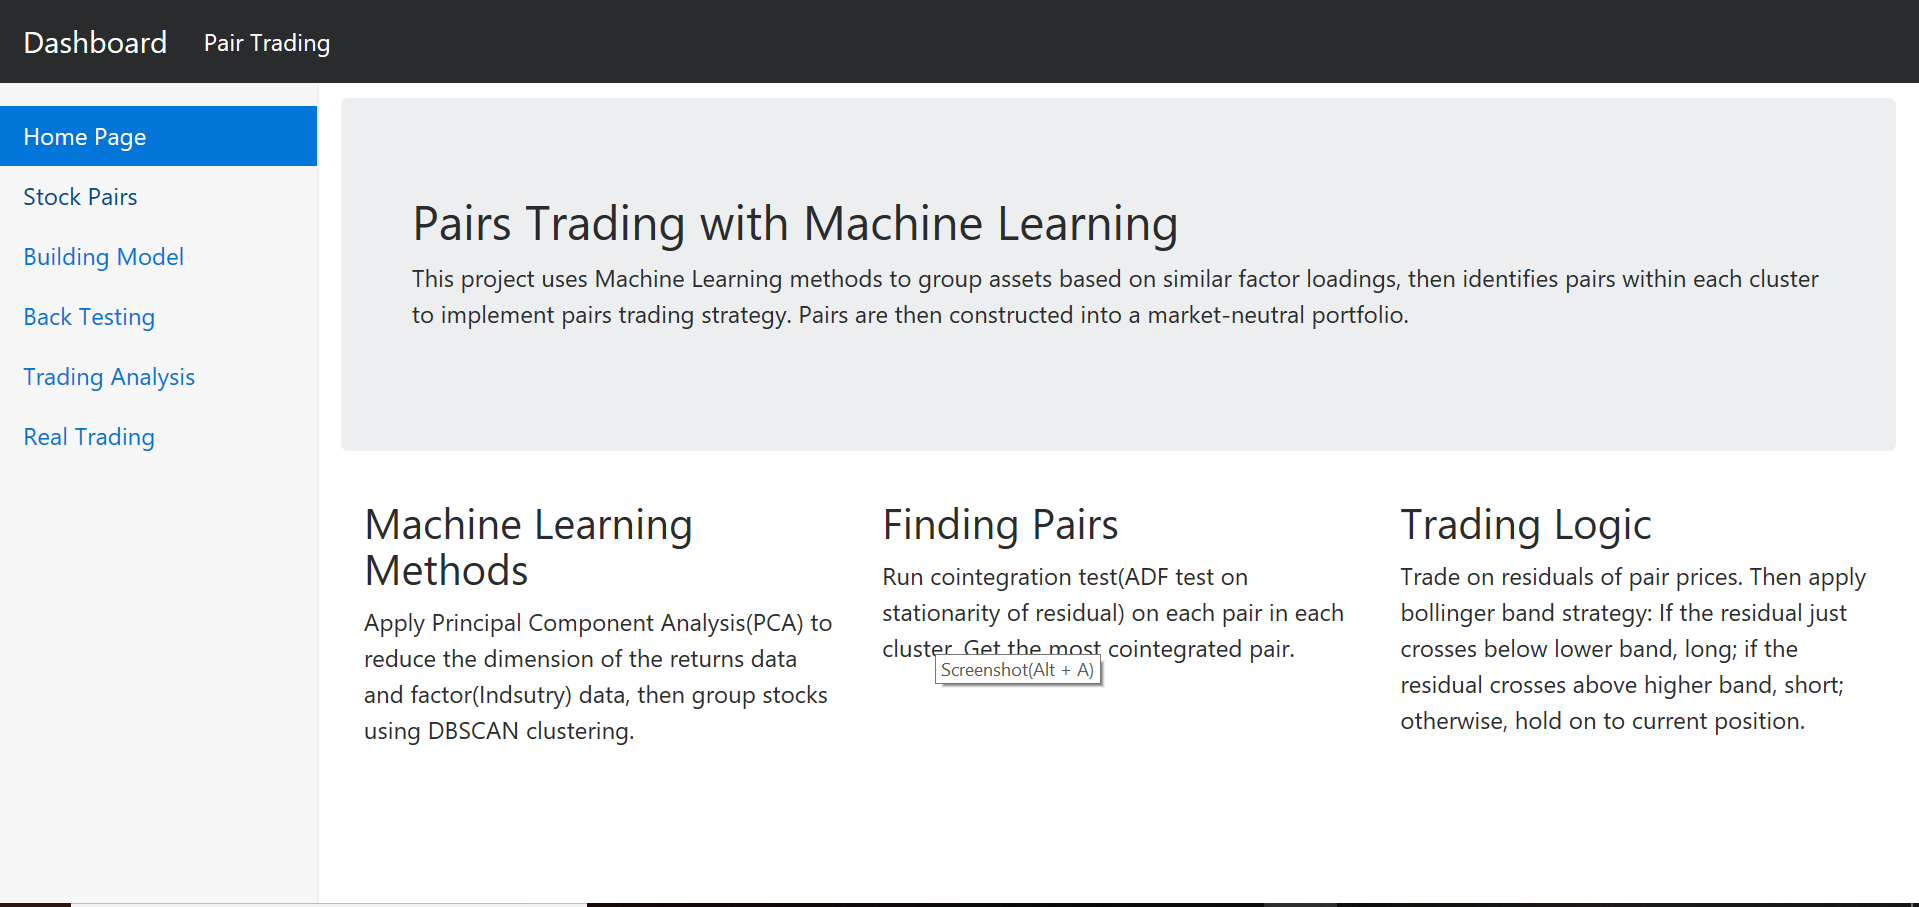
\includegraphics[scale=0.4]{performance_analysis/images/dashboard.png}
\caption{Dashboard Home Page}
\label{fig:dashboard}
\end{figure}



%
%!TEX root = ../thesis.tex
\chapter{Conclusions and Future Work}
\label{chap:conclusions}

This capstone project builds a Python platform that can be used to test quantitative trading models in a network setting under client/server infrastructure with performance analysis displayed on web dashboard. From our backtesting and simulated trading results, we see that the performance of simulated trading is much worse than that of backtesting, although backtesting shows that our trading model has a 2.5 Sharpe ratio and 25\% annual return. It concludes that we should be careful in real-time trading even with a profitable model shown in backtesting and we always want to do paper trading before real trading. 

This python platform is a good tool for testing trading models, alerting for potential losses. However, there are limitations. Our assumptions of order book are simple and our simulated trading is not equivalent to paper trading. Paper trading is to trade based on real-time order books with no real money evolved. Our simulated trading has order book that is simulated from historical data and is fixed for each day. Our order book is too simple as compared to a real order book and is lack of real market dynamics. We would need tick level data to actually simulate a real market, for our first improvement that can be done to this project. Furthermore, we can improve our order matching algorithm and allow for market orders. We always place order at the best bid and offer of one order book of that day and it is always filled at this price. While in the real market, the limit order is fulfilled at our price and better, possibly split into different trades. It also has market order that takes many prices to get as much quantity filled as possible. For our pairs trading model, market orders are more reasonable because we are doing dollar neutral strategy and our purpose is to get all quantity of orders filled.

There are also ways to improve our trading model. First, we have many hyperparameters in our trading model, including training and testing time periods, significance level in adjusted dickey fuller test, number of standard deviations and moving average period in bollinger band construction, number of principle components and epsilon in PCA. These hyperparameters can be optimized through cross validation. Second, we can do kalman filter instead of one simple ordinary least square. Third, we should set up stop loss level to prevent losses as in our simulated trading. Fourth, we should also include transaction costs in our model.

%%%%% Appendices start %%%%%%%%%%%%%%%%
%% Comment out the following line if your thesis has no appendix
\appendix
\chapter{Appendix: Code\label{chap:append}}

%New colors defined below
\definecolor{codegreen}{rgb}{0,0.6,0}
\definecolor{codegray}{rgb}{0.5,0.5,0.5}
\definecolor{codepurple}{rgb}{0.58,0,0.82}
\definecolor{backcolour}{rgb}{0.95,0.95,0.92}

%Code listing style named "mystyle"
\lstdefinestyle{mystyle}{
  backgroundcolor=\color{backcolour},   commentstyle=\color{codegreen},
  keywordstyle=\color{magenta},
  numberstyle=\tiny\color{codegray},
  stringstyle=\color{codepurple},
  basicstyle=\tiny,
  breakatwhitespace=false,         
  breaklines=true,                 
  captionpos=b,                    
  keepspaces=true,                 
  numbers=left,                    
  numbersep=5pt,                  
  showspaces=false,                
  showstringspaces=false,
  showtabs=false,                  
  tabsize=2
}

%"mystyle" code listing set
\lstset{style=mystyle}


\section{Platform Client}
\lstinputlisting[language=Python, caption=Platform Client]{appendix/code/client.py}


\section{Platform Server}
\lstinputlisting[language=Python, caption=Platform Client, basicstyle=\tiny]{appendix/code/server.py}



%% Note: If your thesis has more than one appendix, NYU requires a "list of
%% appendices" page before the body of the thesis. I don't provide the tools
%% to create that here, so you're on your own for that one... Sorry.
%\input{app2}

%%%% Input bibliography file %%%%%%%%%%%%%%%
% %% NYU PhD thesis format. Original template created by José Koiller 2007--2008.
%% Updated by Anshul Vikram Pandey with new design guidelines. 2017-2018

%% Use the first of the following lines during production to
%% easily spot "overfull boxes" in the output. Use the second
%% line for the final version.
\documentclass[12pt,draft,letterpaper]{report}
% \documentclass[12pt,letterpaper]{report}
% \documentclass[12pt]{article}

%% Replace the title, name, advisor name, graduation date and dedication below with
%% your own. Graduation months must be January, May or September.
\newcommand{\thesistitle}{Pairs Trading with Machine Learning on Distributed Python Platform}
\newcommand{\thesisauthor}{Yicheng Wang}
\newcommand{\thesisadvisor}{Song Tang}
\newcommand{\graddate}{May 2019} % like January XX, May 20XX, September 20XX

%% If you do not want a dedication, scroll down and comment out
%% the appropriate lines in this file.
%% \newcommand{\thesisdedication}{To all the Ph.D. pursuing brave souls}

%% The following makes chapters and sections, but not subsections,
%% appear in the TOC (table of contents). Increase to 2 or 3 to
%% make subsections or subsubsections appear, respectively. It seems
%% to be usual to use the "1" setting, however.
\setcounter{tocdepth}{1}

%% Sectional units up to subsubsections are numbered. To number
%% subsections, but not subsubsections, decrease this counter to 2.
\setcounter{secnumdepth}{3}

% Setting a gap between page number and text block


%% Page layout (customized to letter paper and NYU requirements):
\setlength{\oddsidemargin}{.6in}
\setlength{\textwidth}{5.8in}
\setlength{\topmargin}{0.5in}
\setlength{\headheight}{0in}
\setlength{\headsep}{0in}
\setlength{\textheight}{8.3in}
\setlength{\footskip}{.5in}

%% Use the following commands, if desired, during production.
%% Comment them out for final version.
%\usepackage{layout} % defines the \layout command, see below
%\setlength{\hoffset}{-.75in} % creates a large right margin for notes and \showlabels

%% Controls spacing between lines (\doublespacing, \onehalfspacing, etc.):
\usepackage{setspace}

%
%% \usepackage{amsmath}
%% \usepackage{amssymb}
\usepackage{xspace}
\usepackage{algorithmic}
\usepackage{algorithm}
\usepackage{microtype}
\usepackage{subfigure}
\usepackage{color}
\usepackage{url}
\usepackage{fancyhdr}
\usepackage[utf8]{inputenc}
\usepackage[english]{babel}
\usepackage[final]{graphicx}
\usepackage[final]{listings}
\usepackage{color}
% \newfloat{algorithm}{t}{lop}

\pagestyle{fancy}
\fancyhf{}
\renewcommand{\headrulewidth}{0pt}
\fancyhead[LE]{}
\fancyhead[RO]{}
\fancyhead[RE]{}
\fancyhead[LO]{}
\fancyfoot[C]{}
\rhead{\thepage}

\fancypagestyle{plain}{%
\fancyhf{}
\rhead{\thepage}
}

\setlength{\headheight}{20pt} 

%% Use the line below for official NYU version, which requires
%% double line spacing. For all other uses, this is unnecessary,
%% so the line can be commented out.
\onehalfspacing % requires package setspace, invoked above

%% Each of the following lines defines the \com command, which produces
%% a comment (notes for yourself, for instance) in the output file.
%% Example:    \com{this will appear as a comment in the output}
%% Choose (uncomment) only one of the three forms:
%\newcommand{\com}[1]{[/// {#1} ///]}       % between [/// and ///].
\newcommand{\com}[1]{\marginpar{\tiny #1}} % as (tiny) margin notes
%\newcommand{\com}[1]{}                     % suppress all comments.



%% Cross-referencing utilities. Use one or the other--whichever you prefer--
%% but comment out both lines for final version.
%\usepackage{showlabels}
%\usepackage{showkeys}
% \pagestyle{headings}

\begin{document}
%% Produces a test "layout" page, for "debugging" purposes only.
%% Comment out for final version.
%\layout % requires package layout (see above, on this same file)
%% Sets page numbering to "roman style" i, ii, iii, iv, etc:

%%%%%% Cover page %%%%%%%%%%%
%% Sets page numbering to "roman style" i, ii, iii, iv, etc:
\pagenumbering{roman}
\thispagestyle{empty}
\begin{center}
{\bfseries 
  {\large\thesistitle}
  \vspace{1in}
  
 {\large {\bf CAPSTONE}}\\
  \vspace{.5in}
  
  \begin{doublespace}
  {\large  
  Submitted in Partial Fulfillment of\\
  % \vspace{.1in}
  the Requirements for\\
  % \vspace{.1in}
  the Degree of\\}
  \end{doublespace}
  \vspace{.5in}
  
  {\large Master of Science (Finance and Risk Engineering)}\\
  \vspace{.5in}
  
  at the \\
  \vspace{.2in}
  
  {\large
  NEW YORK UNIVERSITY\\
  \vspace{-0.05in}
  TANDON SCHOOL OF ENGINEERING\\
  }
  \vspace{.2in}
  
  by
  \vspace{.5in}

  {\large\thesisauthor}
  \vspace{.5in}
  % \vfill

  {\large\graddate}
}

\end{center}

\newpage

%%%%%%%%%%%%%% Ackknowlegment %%%%%%%%%%%%%%%%%
%% Comment out the following lines if you do not want to acknowledge
%% anyone's help...
\section*{Acknowledgements}
\addcontentsline{toc}{section}{Acknowledgements}
%!TEX root = thesis.tex

I would like to extend my sincere gratitude to Prof. Song Tang for his expert guidance and constructive
feedback throughout the course of this project. I appreciate the patience with which he would tackle my
doubts and the time he would spare from his busy schedule to meet during the course of his work-day
to discuss. His inputs to this project are invaluable. I would also like to thank the Finance and Risk
Engineering department at NYU Tandon School of Engineering to give me the opportunity to work on this advanced topic for my
capstone project, during the course of which I learned a lot.

\noindent
\makebox[\textwidth]{\hfill\makebox[3in]{\hfill Yicheng Wang\hfill}}
\makebox[\textwidth]{\hfill\makebox[3in]{\hfill\graddate\hfill}}


\newpage


%%%%%%%%%%%%%% Abstract %%%%%%%%%%%%%%%%%
\section*{}
\begin{center}
{\bfseries 
  %{\large\thesistitle}
  \vspace{.25in}  
  {\bf ABSTRACT}\\
  \vspace{.25in}
}
\end{center}
\addcontentsline{toc}{section}{Abstract}
%!TEX root = thesis.tex

%
This capstone project implements a distributed Python platform that can be used to test quantitative models for trading financial instruments in a network setting under client/server infrastructure. Normally, we backtest locally using past historical data to check the performance of our trading strategies. The performance result, in this case, is usually an illusion of what the actual performance is in real-time trading. We also show in this paper this conclusion by showing that our quantitative trading model performs much worse in the simulated trading than that in backtesting environment. Therefore, we build this Python platform not only for implementing trading strategies and backtesting them historically but also for simulating trades similar to what is in real market, acting as another control before real-time trading.
\newpage

%%%% Table of Contents %%%%%%%%%%%%
\tableofcontents
% \clearpage
% \pagestyle{headings}


%%%%% Body of thesis starts %%%%%%%%%%%%
\pagenumbering{arabic} % switches page numbering to arabic: 1, 2, 3, etc.

%% Introduction. If your thesis has no introduction, or chapter 1 is
%% meant to be the introduction, then comment out the lines below.
%% \section*{Introduction}\addcontentsline{toc}{section}{Introduction}
%\input{intro}

%%If your thesis has different "Parts", use commands such as the following:
%!TEX root = ../thesis.tex
\chapter{Introduction}
\label{chap:introduction}

%
This capstone project does the following several things coded in Python:
it first sets market data retrieval using Unicorn data feed and parses market data in json format to store market data for backtesting in SQLite database; then implements trading logic; sets up Python Client/Server communication and multi-threading and implements real-time feed to simulate real trade; finally displays trading analysis and PnL on web dashboard. The program has to run in order as described. The program design is also shown in flow chart Figure 1.1.

\begin{figure}
\centering
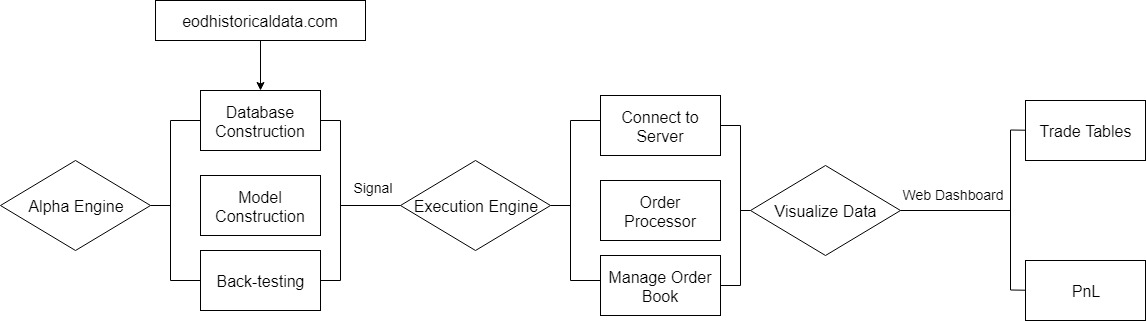
\includegraphics[scale=0.35]{introduction/images/flowchart.jpg}
\caption{Program Design}
\label{fig:flow}
\end{figure}

%
The server is a multi-thread application which coordinates among all the client applications. Its main purposes are 1) messaging among all the participants, 2) maintain a market participant list, and the list of stocks traded by participants, and 3) generate a consolidated order book for all the participants. The client application, also a multi-threading application in network-oriented environment, will communicate with the server. Each application will implement required messages in json format. 

%
Moreover, 1) The sender and receiver threads will support TCP/IP protocol and through Internet sockets;
2) The sender and receiver threads must achieve data synchronization using event and queue;
3) the application will handle direct market data feeds in json format for historical and real-time data from eodhistoricaldata.com;
4) the application will have an integrated database for data persistence. The database we use is sqlite3. We implement tables and SQL statements for our own model buildup, as well as back testing.
5) We will implement a trading model.
6) We manage our own order books and calculate P/L.

%
The trading model is a pairs trading model on stocks in SP500. We use machine learning techniques in selecting pairs. Specifically, we use PCA to reduce dimensions and then DBSCAN clustering to group stocks. We then identify pairs within clusters to implement dollar neutral Bollinger Band pairs trading strategy. Finally, we construct a portfolio with pairs equally weighted. We achieve a 2.5 Sharpe ratio backtested in 2018. However, we can potentially lose money when we trade in simulated market using client/server infrastructure we built.

%
We proceed as follows. In Chapter 2: Background, we provide some backgrounds in pairs trading model and machine learning techniques we used. Chapter 3: Data, we describe how we retrieve, parse and store data into database. In Chapter 4: Trading Model, we describe our trading logic, how we train, build and backtest our model. In Chapter 5: Client/Server, we provide details of client server infrastructure and how they communicate. In Chapter 6: Simulated Trade, we explain how we implement trading strategy to trade in client/server infrastructure. In Chapter 7: Performance Analysis, we show our performance of backtest and simulated trade results and how we move the visualization to web dashboard using flask. At last, we have Chapter 8: Conclusion and appendix where source codes will be provided.

%
%!TEX root = ../thesis.tex
\chapter{Background}
\label{chap:background}
\nocite{*}


\section{Pairs Trading}

Pairs trading is a market-neutral trading strategy that matches a long position with a short position in a pair of highly correlated instruments such as two stocks, exchange-traded funds (ETFs), currencies, commodities or options. Pairs traders wait for weakness in the correlation and then go long the under-performer while simultaneously short selling the over-performer, closing the positions as the relationship returns to statistical norms.\cite{investo:pairs}


\subsection{Cointegration Test}

In order to find pairs to trade in pairs trading, we look for cointegrated relationship in pairs. A pair is cointegrated if individual instruments are of same order and the linear combination of them is stationary. We test stationarity of the linear combination of the pair, say \(y_t\). Stationarity is referred as weak stationarity in this case that a series is stationary if the mean and autocovariance are independent of time and the variance is finite for all times.\cite{wiki:stationarity} We simply regress \(y_t\) on its lagged values \(y_{t-1}\) and find out whether the coefficient \(\phi\) is 1 or not. Consider autoregressive process of order 1, AR(1), as shown:\cite{study:coint}
\begin{equation}
y_t = \phi y_{t-1} + \epsilon_t
\end{equation}
where \(\epsilon_t\) is white noise error term with mean zero and constant variance. Then,
\begin{equation}
\Delta y_t = \delta y_{t-1} + \epsilon_t
\end{equation}
where \(\Delta\) is first difference and \(\delta = \phi - 1\). If \(\delta = 0\), then \(\Delta y_t = \epsilon_t \), it means \(y_t\) is random walk and non-stationary. Otherwise, it is a stationary process. This is called Dickey-Fuller Test.

Moreoever, we have Augmented Dickey-Fuller (ADF) Test, which allows for higher-order autoregressive processes, as shown:\cite{study:coint}
\begin{equation}
\Delta y_t = \alpha + \beta t + \gamma y_{t-1} + \sum_{j=1}^{p} \delta_j \Delta y_{t-j} + \epsilon_t
\end{equation}

For this model, we test for the null hypothesis as \(H_0: \gamma = 0\) against alternative hypothesis as \(H_1: \gamma < 0\). We reject the null if the test statistic is smaller than critical value of a significance level. 

In this project, we use ADF test to check cointegration of two stock price series. We construct linear combination of two stock price series as:
\begin{equation}
y_t = S_t^1 - a S_t^2
\end{equation}
where \(S_t^1\) and \(S_t^2\) are price series of stock 1 and stock 2.


\subsection{Bollinger Band Strategy}

Bollinger band strategy is typically used in pairs trading to capture profit between upper and lower bands. Upper and lower band are constructed 1-2 standard deviations from the moving average of the series \(y_t\).\cite{pairstrading} There are also many ways of entry and exit, long and short. In our trading model, we long when \(y_t\) crosses down the lower band, short when \(y_t\) crosses up the upper band, where the profit is captured between buy and sell points, as shown in Figure 2.1.

\begin{figure}[h!]
\centering
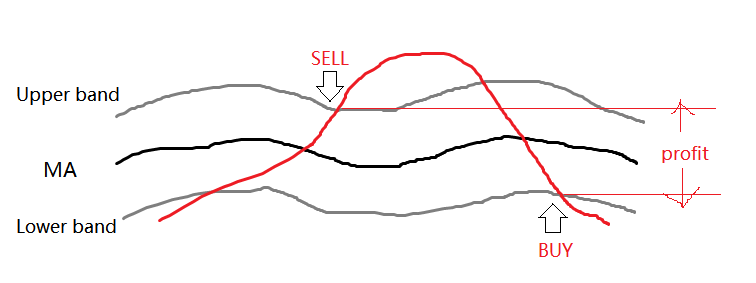
\includegraphics{background/images/bollinger.png}
\caption{Bollinger Band}
\label{fig:bollinger}
\end{figure}



\section{Machine Learning}

\subsection{Principle Component Analysis}

Principle Component Analysis (PCA) is used for reducing the number of variables comprising a dataset while retaining the variability in the data, or identifying hidden patterns in the data, and classifying them according to how much of the information, stored in the data, they account for.\cite{pca} We use PCA for our stock market data for both purposes. 

We take stock price panel data as score matrix \(A\), and coefficient vector \(l\) that generates linear combination on \(A\) which yields principle components \(Y\) of smaller dimension than \(A\). Principle components \(Y\) are independent and each coefficient vector \(l_i\) is required to maximize the variance of its corresponding principle component \(Y_i\), as shown:\cite{pca}
\begin{equation}
\max{Var(Y_i) = l_i^T C l_i}
\end{equation}
\[s.t.\]
\[||l_i^T|| = 1, \forall i\]
\[l_i^T l_j = 0, \forall j\neq i\]
which has Lagrangian form:
\begin{equation}
L(l_i, \lambda_i, \delta) = l_i^T C l_i - \lambda_i(l_i^T l_i - 1) - \delta(l_i^T l_i)
\end{equation}
Maximizing L by taking partial derivatives to 0, we obtain \(C l_i = \lambda_i l_i\), where \(C\) is covariance matrix of \(A\) and \(\lambda_i, l_i\) are corresponding eigenvalues and eigenvectors. 

Therefore, principle components are constructed from eigenvectors of score matrix with score matrix itself: \(Y_i = l_i^T A\).


\subsection{DBSCAN Clustering}

\begin{figure}[h!]
\centering
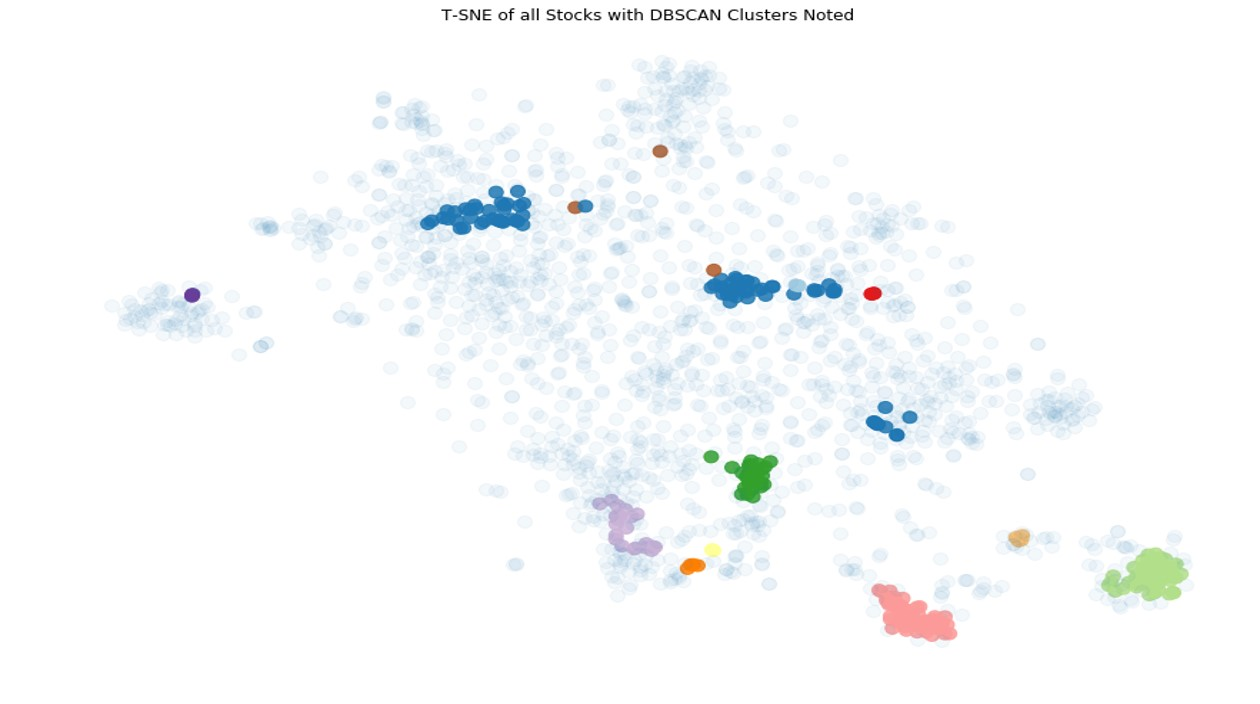
\includegraphics[scale=0.4]{background/images/Clustering.jpg}
\caption{DBSCAN Clustering}
\label{fig:cluster}
\end{figure}

Density-based spatial clustering of applications with noise (DBSCAN) is a density-based clustering non-parametric algorithm: given a set of points in some space, it groups together points that are closely packed together (points with many nearby neighbors).\cite{wiki:dbscan} Unlike normal clustering method that group all points, DBSCAN does not group outliers that lie alone in low-density regions. Another characteristic of DBSCAN is that it is likely to produce different clusters at each run. An example is shown in Figure 2.1.

DBSCAN has two important hyperparameters. Minimum sample size is minimum number of points in a group. Distance parameter is largest distance between points in a group. We pick \( \epsilon = 1.8, min samples = 3\) to get a reasonable number of resulting clusters, which is about 8 clusters.


%
%!TEX root = ../thesis.tex
\chapter{Data}
\label{chap:data}


\section{Data Information}

\subsection{Data Tables}
\begin{enumerate}
    \item "TickerName": stock market data from eodhistoricaldata and are in json format, shown in figure 3.2 includes symbol, date, open, high, low, close, adjusted close, volume from 2014-01-01 to recent, where only adjusted close price is used in our trading model.
    \item "sp500": SP500 constituent data from pkgstore.datahub.io in json format, shown in figure 3.1, which includes name, sector and symbol.
    \item "stockpairs": stock pairs constituent data from training model, which includes ticker1 and ticker2 in pairs, score that represent the strength of cointegration, profit and loss for the pair in backtesting.
    \item "pairprices": stock pairs price data with adjusted close price of each pair from stock market data, residuals from pair prices regression, and bollinger band constructed from residuals.
    \item "trades": trades data that record pair, date, price, quantity and PnL of trade status everyday.
\end{enumerate}

\subsection{Data Retrieval}
We first put SP500 constituent data into database, then retrieve data from each ticker from SP500 and also SP500 index price.

\begin{figure}
\centering
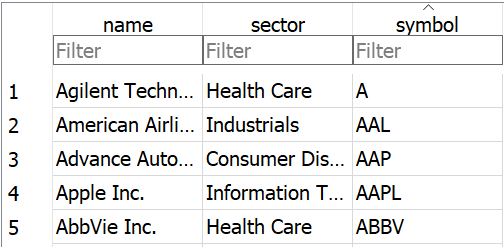
\includegraphics[scale=0.6]{data/images/sp500table.png}
\caption{Table: SP500 Constituents}
\label{fig:sp500}
\end{figure}

\begin{figure}
\centering
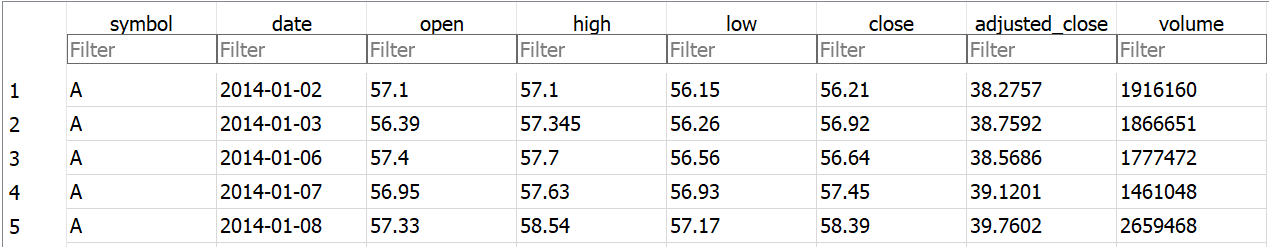
\includegraphics[scale=0.6]{data/images/A.png}
\caption{Table: Stock A}
\label{fig:stockA}
\end{figure}

Function get\_daily\_data() takes in ticker name, start date, end date, data url, api key to get market data for one stock starting from start date to end date. Python packpage urlopen is used to open url and data is parsed from json format to dictionary then to pandas dataframe in Function download\_stock\_data(). Then, the dataframe is stored in SQLite in this function. These functions are shown in Figure 3.3 and 3.4.

\begin{figure}
\centering
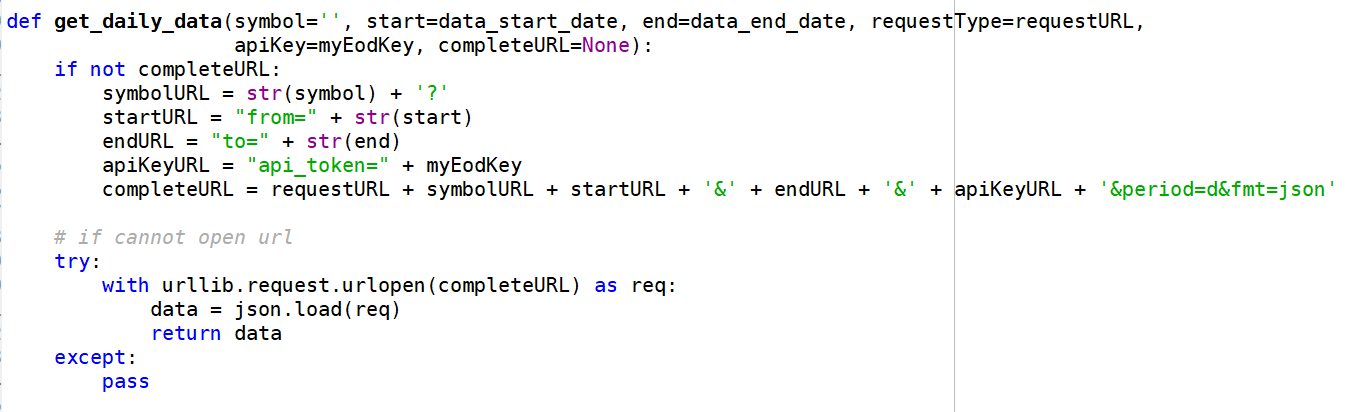
\includegraphics[scale=0.6]{data/images/getdailydata.png}
\caption{Function: get\_daily\_data()}
\label{fig:getdailydata}
\end{figure}

\begin{figure}
\centering
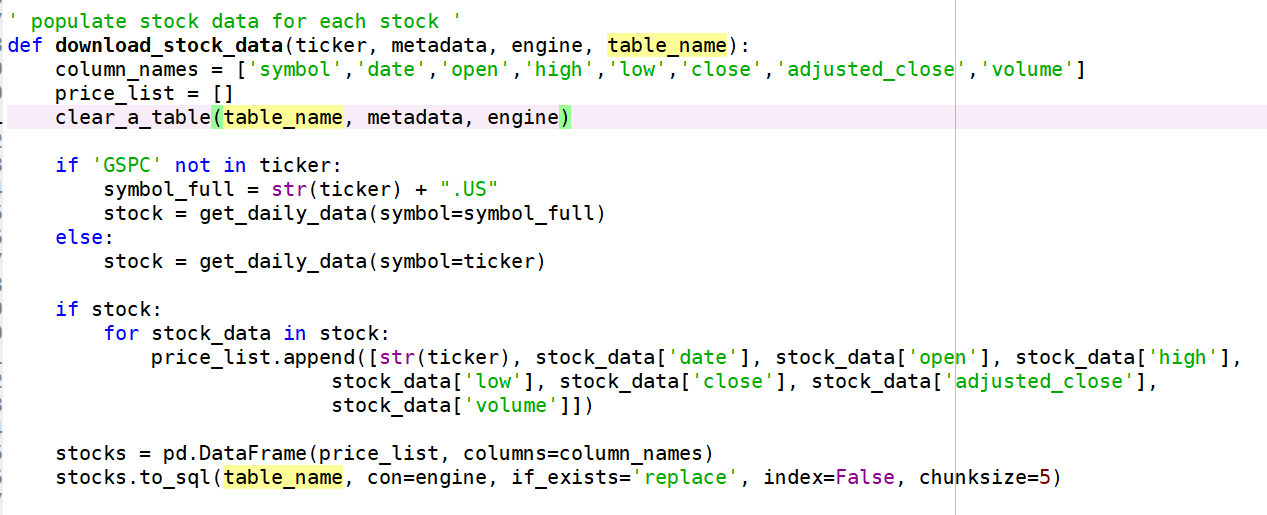
\includegraphics[scale=0.6]{data/images/downloaddata.png}
\caption{Function: download\_stock\_data()}
\label{fig:downloaddata}
\end{figure}


\section{Database Design}

Our database design comprises of 504 tables with two entity relationship, as shown in Figure 3.1. First, each of 500 ticker database with "symbol" and "date" as primary key and "symbol" as foreign key maps to "name" as primary key from sp500 constituents database. Second, table "pairprices" and table "trades" both have "symbol1", "symbol2" that reference to "ticker1", "ticker2" in table stockpairs.

\begin{figure}[h!]
\centering
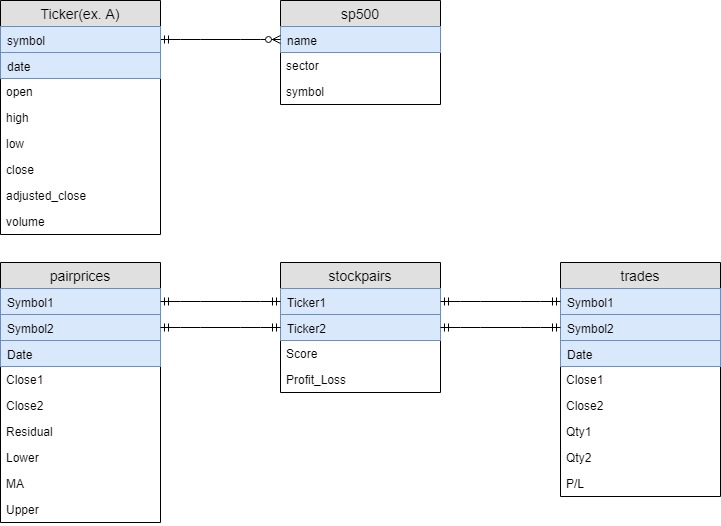
\includegraphics[scale=0.45]{data/images/database.jpg}
\caption{Database Design}
\label{fig:database}
\end{figure}

%
%!TEX root = ../thesis.tex
\chapter{Trading Model}
\label{chap:trading model}

Our trading model is pairs trading model. Pairs are constructed from cointegrated stocks in SP500 stocks in function training\_model(). Then, each pairs is to implement bollinger band strategy in function building\_model(). Later, our trading model will enter function backtesting() with trading signals and corresponding PnL.

\section{Training}

\subsection{Parameters}
\begin{itemize}
    \item training start date: 2014-01-01, training end date: 2018-01-01
    \item capital: 1,000,000 for each pair
    \item cointegration: significance = 0.05
    \item Bollinger Band: standard deviation = 2, moving average period = 10
    \item PCA: principle components = 50, epsilon = 1.8, minimum sample = 3
\end{itemize}

\subsection{Steps}
\begin{enumerate}
    \item 500 stocks price return data of 4 years are reduced to 50 principle components using PCA (background in Section 2.2.1). The resulting dataframe is then in 50 * 500 dimension.
    \item We apply DBSCAN Clustering (background in 2.2.2) to group stocks according to 50 principle components. It will result in 6 to 10 groups with minimum of 3 stocks per group.
    \item Pairs are selected within each group. In each group, every two stocks go through cointegration test (background in 2.1.1). As shown in Figure 4.1, only pairs that pass the test most significantly (smallest p-value, or largest t-statistics) in each group are selected. Information about pairs are stored in table "stockpairs". As shown in Figure 4.2, all pairs have large score (t-statistics).
    \item We then regress one stock price series to another stock price series for each pair using training data. Residual is then constructed in this way as in Equation (2.4). Later, we build bollinger band using residuals (background in Section 2.1.2). Pairs prices, residuals and bollinger bands data are stored in table "pairprices". 
\end{enumerate}

\begin{figure}
\centering
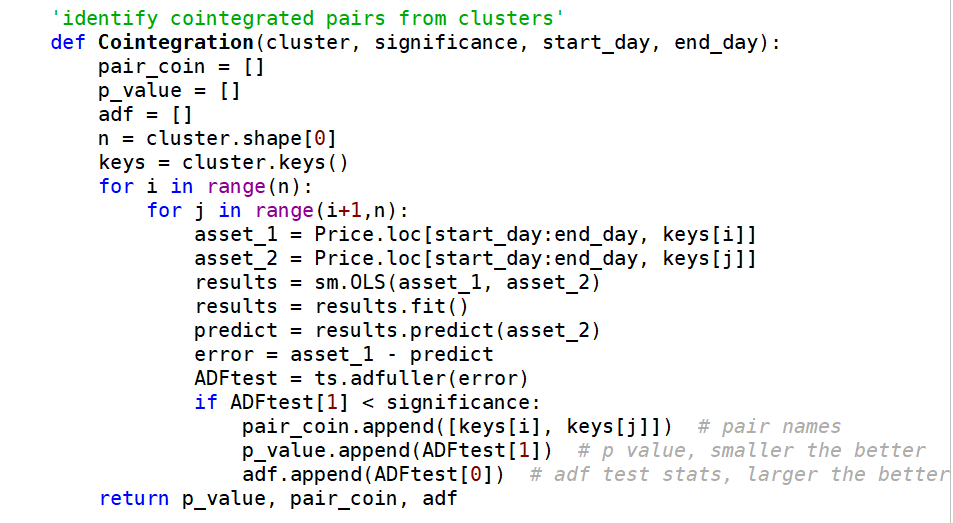
\includegraphics[scale=0.6]{model/images/cointegration.png}
\caption{Function: Cointegration()}
\label{fig:cointegration}
\end{figure}

\begin{figure}[h!]
\centering
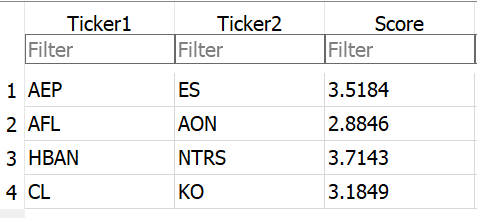
\includegraphics[scale=0.8]{model/images/stockpairs.png}
\caption{Table: Stockpairs}
\label{fig:stockpairs}
\end{figure}




\section{Backtesting}

We backtest from 2018-01-01 to 2019-01-01 for one year. A class is constructed for each stock pair shown in Figure 4.3, where trade is created with stock pair data of each day and is updated if there is a trading signal. Each pair is assigned with equal capital and is market neutral. Profit and loss is also calculated daily according current position and price. Backtesting result is stored in table "trades".


\begin{figure}[h!]
\centering
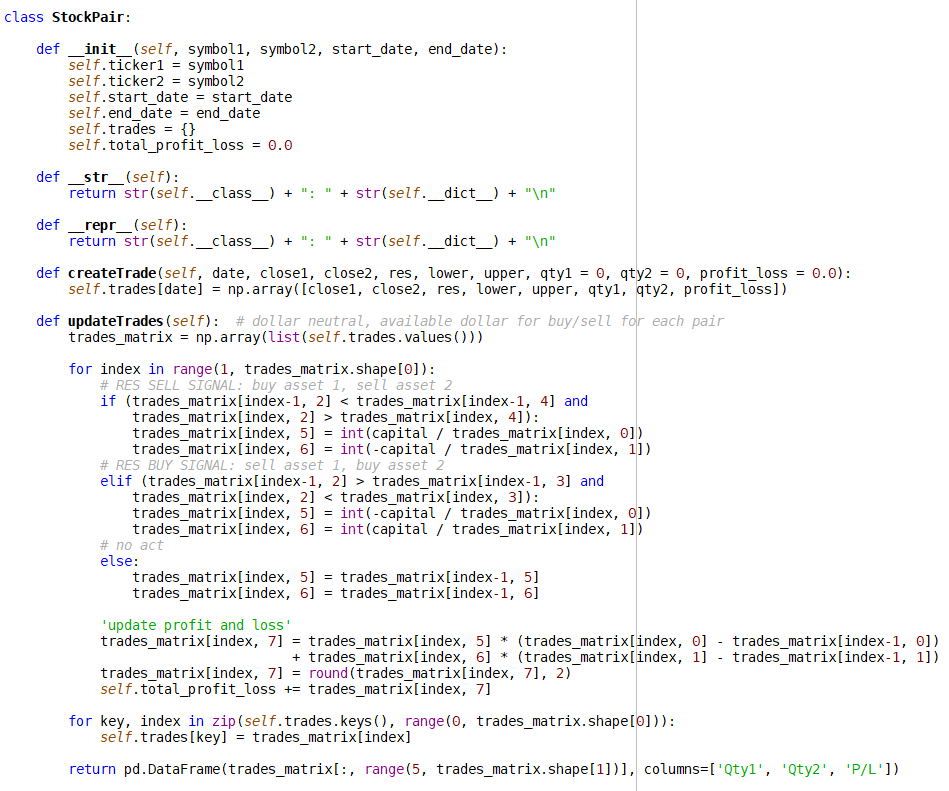
\includegraphics[scale=0.8]{model/images/class.png}
\caption{Class: StockPair}
\label{fig:class}
\end{figure}



%
%!TEX root = ../thesis.tex
\chapter{Client Server}
\label{chap:client server}


The sender and receiver threads will support TCP/IP protocol and through Internet sockets. Server will wait for connection from client, will receive and process messages from client, and will process the request and send back response if client ask for. Socket diagram is shown in Figure 5.1.

\begin{figure}[h!]
\centering
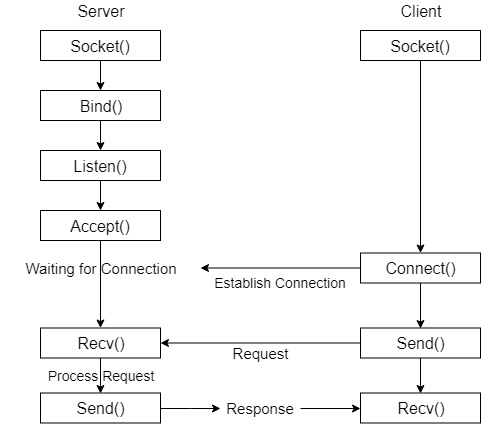
\includegraphics[scale=0.5]{client_server/images/socket.jpg}
\caption{Socket Diagram}
\label{fig:socket}
\end{figure}

The sender and receiver threads achieve data synchronization using event and queue. When the client sends a request message to the server, server returns a message queue while the client is waiting for it. Whenever this event is set, data in queue  will be available to the client. This synchronization process is shown in Figure 5.2.

\begin{figure}[h!]
\centering
\includegraphics[scale=0.5]{client_server/images/event.png}
\caption{Synchronization Process Diagram}
\label{fig:synch}
\end{figure}


\section{Order Book}
    
Server will provide consolidated books for 30 trading days: 
\begin{enumerate}
    \item Simulated from market data starting from 1/2/2019.
    \item Order book is consist of: order index, symbol, side (buy or sell), price, quantity, and order status, shown in Figure 5.3.
    \item Each simulated trading date has one new book for every 30 seconds from daily historical data, with buy orders and sell orders simulated from the high and low price from the day, with price step of 0.05 and daily volume randomly distributed cross all price points. 
    \item Each simulated trading day lasts 30 seconds, following by 5 seconds of pending closing phase and 5 seconds of market closed phase before market reopen. There are 5 phases of market: 
    \begin{enumerate}
        \item Not Open, start of simulated trading
        \item Pending Open, 
        \item Open, 30s
        \item Pending Close, 5s
        \item Market Close, 5s
    \end{enumerate}
    \item The book supports partial fill, based on comparison of order quantity and available quantity on the book. The order status could be New, Filled or Partial Filled.
    \item If the market status is pending close, trade price will be worse by 0.01.
    \item All orders placed are limit orders.
\end{enumerate}

\begin{figure}[h!]
\centering
\includegraphics[scale=0.8]{client_server/images/orderbook.png}
\caption{Order Book}
\label{fig:order}
\end{figure}


%
%!TEX root = ../thesis.tex
\chapter{Simulated Trading}
\label{chap:simulated trading}


After training, building, and backtesting the trading model, we will start simulated trading with a "real-time" data feed for 30 days, starting from 01/02/2019. Every 40 seconds, there is a market data feed of another day read from "eodhistoricaldata.com". 

During simulated trading, first, it will logon to that includes a list of stocks from our trading model. Then it will loop to get market status until market open. It will send orders to server only during market open and pending closing. It will get order book information given a list of stocks to access the best available prices. Function get\_orders() tries to get the trading signal using latest data and trained model, then orders are placed and traded if there is any signal on that day. After placing orders, a new day will start every 40 seconds. Then we loop to get market status and repeat this process again.

Finally, when 30 days passed, we quit client and server connection and start to do trading analysis, which will be published to web dashboard. We design an algorithm to detect the ending of 30-day trading period: we will quit the connection whenever the market status remain in "Close" for more than 150 seconds. 

The flowchart of trading under network setting is shown in Figure 6.1.

\begin{figure}[h!]
\centering
\includegraphics[scale=0.5]{simulated_trading/images/trading.jpg}
\caption{Trading Under Network Setting Flowchart}
\label{fig:trading}
\end{figure}

%
%!TEX root = ../thesis.tex
\chapter{Performance Analysis}
\label{chap:performance analysis}

\section{PnL}
According to Figure 6.1, after both backtesting and simulated trading, we have trading analyses that will be displayed on the web dashboard. Figure 7.2 shows the backtesting result. We can see that backtested from 2018 to 2019, we have a profit of over 1 million, which is about 25\% profit, starting with 1 million capital for each pair and 4 millions in total. All 4 pairs trades are profitable and the hit ratio is 100\%. The maximum drawdown is about only 3\%. The resulting Sharpe ratio is 2.5.

Cummulative PnL plot is also shown in Figure 6.2. Performance of our pairs trading model is much better than SP500 performance. The backtesting result shows that our trading model is very profitable, which is a contrast to our simulated trading result in Figure 6.4. There are several reasons that result in huge losses. First and the most important, our pairs trading model fails since pairs have different relationships during the first month of 2019 than the training data. SP500 index movement in 2018 is quite mean-reverting, where its constituents might also have stable relationships in this year. However, SP500 index at the start of 2019 is more momentum, where its constituents are likely to result in different relationships than in 2018. Second, we have flaws in our design of order book and order matching algorithm. Third, our trading model does not have stop loss. Further discussions of these issues and potential improvements are in conclusion.

\begin{figure}[h!]
\centering
\includegraphics[scale=0.5]{performance_analysis/images/pnl1.png}
\caption{Backtesting Statistics}
\label{fig:backteststats}
\end{figure}

\begin{figure}
\centering
\includegraphics[scale=0.45]{performance_analysis/images/backtest_pnl.jpg}
\caption{Backtesting PnL}
\label{fig:backtest}
\end{figure}

\begin{figure}
\centering
\includegraphics[scale=0.45]{performance_analysis/images/trade_pnl.jpg}
\caption{Simulated Trading PnL}
\label{fig:trading}
\end{figure}



\section{Web Dashboard}

Our web dashboard is built through flask. There are several modules on the web dashboard:
\begin{itemize}
    \item Home Page: displays our pairs trading strategy logic, shown in Figure 7.4;
    \item Stock Pairs: displays Table stockspairs;
    \item Building Model: displays Table pairprices;
    \item Back Testing: displays Table trades;
    \item Trading Analysis: displays performance analysis table and plotted PnL for backtesting result;
    \item Real Trading: displays performance analysis table and plotted PnL for simulated tradingg result;
\end{itemize}

Whenever a module button is clicked on the page, the program will run on the server/client side and the display will show when the process is finished. Each module has to run in order. For "Real Trading" module, it will wait for over 10 minutes until the performance result shows on the page. 

Flask will run on the main thread with the client side. We have another thread called client thread that will do simulated trading part with client/server communication. To do that, we need a global variable "bClientThreadStarted" to keep track if client thread start. It is set to false initially, and to true whenever simulated trading starts. The main thread will wait for client thread finishes to continue.

\begin{figure}
\centering
\includegraphics[scale=0.4]{performance_analysis/images/dashboard.png}
\caption{Dashboard Home Page}
\label{fig:dashboard}
\end{figure}



%
%!TEX root = ../thesis.tex
\chapter{Conclusions and Future Work}
\label{chap:conclusions}

This capstone project builds a Python platform that can be used to test quantitative trading models in a network setting under client/server infrastructure with performance analysis displayed on web dashboard. From our backtesting and simulated trading results, we see that the performance of simulated trading is much worse than that of backtesting, although backtesting shows that our trading model has a 2.5 Sharpe ratio and 25\% annual return. It concludes that we should be careful in real-time trading even with a profitable model shown in backtesting and we always want to do paper trading before real trading. 

This python platform is a good tool for testing trading models, alerting for potential losses. However, there are limitations. Our assumptions of order book are simple and our simulated trading is not equivalent to paper trading. Paper trading is to trade based on real-time order books with no real money evolved. Our simulated trading has order book that is simulated from historical data and is fixed for each day. Our order book is too simple as compared to a real order book and is lack of real market dynamics. We would need tick level data to actually simulate a real market, for our first improvement that can be done to this project. Furthermore, we can improve our order matching algorithm and allow for market orders. We always place order at the best bid and offer of one order book of that day and it is always filled at this price. While in the real market, the limit order is fulfilled at our price and better, possibly split into different trades. It also has market order that takes many prices to get as much quantity filled as possible. For our pairs trading model, market orders are more reasonable because we are doing dollar neutral strategy and our purpose is to get all quantity of orders filled.

There are also ways to improve our trading model. First, we have many hyperparameters in our trading model, including training and testing time periods, significance level in adjusted dickey fuller test, number of standard deviations and moving average period in bollinger band construction, number of principle components and epsilon in PCA. These hyperparameters can be optimized through cross validation. Second, we can do kalman filter instead of one simple ordinary least square. Third, we should set up stop loss level to prevent losses as in our simulated trading. Fourth, we should also include transaction costs in our model.

%%%%% Appendices start %%%%%%%%%%%%%%%%
%% Comment out the following line if your thesis has no appendix
\appendix
\chapter{Appendix: Code\label{chap:append}}

%New colors defined below
\definecolor{codegreen}{rgb}{0,0.6,0}
\definecolor{codegray}{rgb}{0.5,0.5,0.5}
\definecolor{codepurple}{rgb}{0.58,0,0.82}
\definecolor{backcolour}{rgb}{0.95,0.95,0.92}

%Code listing style named "mystyle"
\lstdefinestyle{mystyle}{
  backgroundcolor=\color{backcolour},   commentstyle=\color{codegreen},
  keywordstyle=\color{magenta},
  numberstyle=\tiny\color{codegray},
  stringstyle=\color{codepurple},
  basicstyle=\tiny,
  breakatwhitespace=false,         
  breaklines=true,                 
  captionpos=b,                    
  keepspaces=true,                 
  numbers=left,                    
  numbersep=5pt,                  
  showspaces=false,                
  showstringspaces=false,
  showtabs=false,                  
  tabsize=2
}

%"mystyle" code listing set
\lstset{style=mystyle}


\section{Platform Client}
\lstinputlisting[language=Python, caption=Platform Client]{appendix/code/client.py}


\section{Platform Server}
\lstinputlisting[language=Python, caption=Platform Client, basicstyle=\tiny]{appendix/code/server.py}



%% Note: If your thesis has more than one appendix, NYU requires a "list of
%% appendices" page before the body of the thesis. I don't provide the tools
%% to create that here, so you're on your own for that one... Sorry.
%\input{app2}

%%%% Input bibliography file %%%%%%%%%%%%%%%
% %% NYU PhD thesis format. Original template created by José Koiller 2007--2008.
%% Updated by Anshul Vikram Pandey with new design guidelines. 2017-2018

%% Use the first of the following lines during production to
%% easily spot "overfull boxes" in the output. Use the second
%% line for the final version.
\documentclass[12pt,draft,letterpaper]{report}
% \documentclass[12pt,letterpaper]{report}
% \documentclass[12pt]{article}

%% Replace the title, name, advisor name, graduation date and dedication below with
%% your own. Graduation months must be January, May or September.
\newcommand{\thesistitle}{Pairs Trading with Machine Learning on Distributed Python Platform}
\newcommand{\thesisauthor}{Yicheng Wang}
\newcommand{\thesisadvisor}{Song Tang}
\newcommand{\graddate}{May 2019} % like January XX, May 20XX, September 20XX

%% If you do not want a dedication, scroll down and comment out
%% the appropriate lines in this file.
%% \newcommand{\thesisdedication}{To all the Ph.D. pursuing brave souls}

%% The following makes chapters and sections, but not subsections,
%% appear in the TOC (table of contents). Increase to 2 or 3 to
%% make subsections or subsubsections appear, respectively. It seems
%% to be usual to use the "1" setting, however.
\setcounter{tocdepth}{1}

%% Sectional units up to subsubsections are numbered. To number
%% subsections, but not subsubsections, decrease this counter to 2.
\setcounter{secnumdepth}{3}

% Setting a gap between page number and text block


%% Page layout (customized to letter paper and NYU requirements):
\setlength{\oddsidemargin}{.6in}
\setlength{\textwidth}{5.8in}
\setlength{\topmargin}{0.5in}
\setlength{\headheight}{0in}
\setlength{\headsep}{0in}
\setlength{\textheight}{8.3in}
\setlength{\footskip}{.5in}

%% Use the following commands, if desired, during production.
%% Comment them out for final version.
%\usepackage{layout} % defines the \layout command, see below
%\setlength{\hoffset}{-.75in} % creates a large right margin for notes and \showlabels

%% Controls spacing between lines (\doublespacing, \onehalfspacing, etc.):
\usepackage{setspace}

%
%% \usepackage{amsmath}
%% \usepackage{amssymb}
\usepackage{xspace}
\usepackage{algorithmic}
\usepackage{algorithm}
\usepackage{microtype}
\usepackage{subfigure}
\usepackage{color}
\usepackage{url}
\usepackage{fancyhdr}
\usepackage[utf8]{inputenc}
\usepackage[english]{babel}
\usepackage[final]{graphicx}
\usepackage[final]{listings}
\usepackage{color}
% \newfloat{algorithm}{t}{lop}

\pagestyle{fancy}
\fancyhf{}
\renewcommand{\headrulewidth}{0pt}
\fancyhead[LE]{}
\fancyhead[RO]{}
\fancyhead[RE]{}
\fancyhead[LO]{}
\fancyfoot[C]{}
\rhead{\thepage}

\fancypagestyle{plain}{%
\fancyhf{}
\rhead{\thepage}
}

\setlength{\headheight}{20pt} 

%% Use the line below for official NYU version, which requires
%% double line spacing. For all other uses, this is unnecessary,
%% so the line can be commented out.
\onehalfspacing % requires package setspace, invoked above

%% Each of the following lines defines the \com command, which produces
%% a comment (notes for yourself, for instance) in the output file.
%% Example:    \com{this will appear as a comment in the output}
%% Choose (uncomment) only one of the three forms:
%\newcommand{\com}[1]{[/// {#1} ///]}       % between [/// and ///].
\newcommand{\com}[1]{\marginpar{\tiny #1}} % as (tiny) margin notes
%\newcommand{\com}[1]{}                     % suppress all comments.



%% Cross-referencing utilities. Use one or the other--whichever you prefer--
%% but comment out both lines for final version.
%\usepackage{showlabels}
%\usepackage{showkeys}
% \pagestyle{headings}

\begin{document}
%% Produces a test "layout" page, for "debugging" purposes only.
%% Comment out for final version.
%\layout % requires package layout (see above, on this same file)
%% Sets page numbering to "roman style" i, ii, iii, iv, etc:

%%%%%% Cover page %%%%%%%%%%%
%% Sets page numbering to "roman style" i, ii, iii, iv, etc:
\pagenumbering{roman}
\thispagestyle{empty}
\begin{center}
{\bfseries 
  {\large\thesistitle}
  \vspace{1in}
  
 {\large {\bf CAPSTONE}}\\
  \vspace{.5in}
  
  \begin{doublespace}
  {\large  
  Submitted in Partial Fulfillment of\\
  % \vspace{.1in}
  the Requirements for\\
  % \vspace{.1in}
  the Degree of\\}
  \end{doublespace}
  \vspace{.5in}
  
  {\large Master of Science (Finance and Risk Engineering)}\\
  \vspace{.5in}
  
  at the \\
  \vspace{.2in}
  
  {\large
  NEW YORK UNIVERSITY\\
  \vspace{-0.05in}
  TANDON SCHOOL OF ENGINEERING\\
  }
  \vspace{.2in}
  
  by
  \vspace{.5in}

  {\large\thesisauthor}
  \vspace{.5in}
  % \vfill

  {\large\graddate}
}

\end{center}

\newpage

%%%%%%%%%%%%%% Ackknowlegment %%%%%%%%%%%%%%%%%
%% Comment out the following lines if you do not want to acknowledge
%% anyone's help...
\section*{Acknowledgements}
\addcontentsline{toc}{section}{Acknowledgements}
\input{acknowledge}
\newpage


%%%%%%%%%%%%%% Abstract %%%%%%%%%%%%%%%%%
\section*{}
\begin{center}
{\bfseries 
  %{\large\thesistitle}
  \vspace{.25in}  
  {\bf ABSTRACT}\\
  \vspace{.25in}
}
\end{center}
\addcontentsline{toc}{section}{Abstract}
\input{abstract}
\newpage

%%%% Table of Contents %%%%%%%%%%%%
\tableofcontents
% \clearpage
% \pagestyle{headings}


%%%%% Body of thesis starts %%%%%%%%%%%%
\pagenumbering{arabic} % switches page numbering to arabic: 1, 2, 3, etc.

%% Introduction. If your thesis has no introduction, or chapter 1 is
%% meant to be the introduction, then comment out the lines below.
%% \section*{Introduction}\addcontentsline{toc}{section}{Introduction}
%\input{intro}

%%If your thesis has different "Parts", use commands such as the following:
\input{introduction/introduction}

%
\input{background/background}

%
\input{data/data}

%
\input{model/model.tex}

%
\input{client_server/client_server}

%
\input{simulated_trading/simulated_trading}

%
\input{performance_analysis/performance_analysis}

%
\input{conclusions/conclusions}

%%%%% Appendices start %%%%%%%%%%%%%%%%
%% Comment out the following line if your thesis has no appendix
\appendix
\input{appendix/app1}

%% Note: If your thesis has more than one appendix, NYU requires a "list of
%% appendices" page before the body of the thesis. I don't provide the tools
%% to create that here, so you're on your own for that one... Sorry.
%\input{app2}

%%%% Input bibliography file %%%%%%%%%%%%%%%
% \input{thesis}
\bibliographystyle{abbrv}
\bibliography{biblio,background/background} % add intelligently

\end{document}

\bibliographystyle{abbrv}
\bibliography{biblio,background/background} % add intelligently

\end{document}

\bibliographystyle{abbrv}
\bibliography{biblio,background/background} % add intelligently

\end{document}

\bibliographystyle{abbrv}
\bibliography{biblio,background/background} % add intelligently

\end{document}
